
\documentclass{aa}  

%
\usepackage{graphicx}
\usepackage[table]{xcolor}
%%%%%%%%%%%%%%%%%%%%%%%%%%%%%%%%%%%%%%%%
\usepackage{txfonts}
\usepackage{bm}
\usepackage{multirow, makecell}
\usepackage{booktabs}
\usepackage{fontawesome}
\newcommand{\github}{\href{https://github.com/dlanzieri/WL_Implicit-Inference}{\faGithub}} %For Denise: Remember to label the final version of the Github repo with the notebook
%%%%%%%%%%%%%%%%%%%%%%%%%%%%%%%%%%%%%%%%

\usepackage[colorlinks=true,citecolor=blue,linkcolor=blue,urlcolor=blue]{hyperref}
\begin{document} 

\title{Optimal Neural Summarisation for Full-Field Implicit Inference by Density Estimation }

\newcommand{\justine}[1]{{\color{cyan}JZ: #1}}
\newcommand{\denise}[1]{{\color{red}DL: #1}}
\newcommand{\FL}[1]{{\color{magenta}FL: #1}}
\newcommand{\LM}[1]{{\color{olive}LM: #1}}

\author{Denise Lanzieri \inst{1}
\and
Justine Zeghal \inst{2}
\and
T. Lucas Makinen \inst{3}
\and
Alexandre Boucaud \inst{2}
\and
Fran\c{c}ois Lanusse \inst{4}
\and
Jean-Luc Starck \inst{4}
}
\institute{Université Paris Cité, Université Paris-Saclay, CEA, CNRS, AIM, F-91191, Gif-sur-Yvette, France
\and
Université Paris Cité, CNRS, Astroparticule et Cosmologie, F-75013 Paris, France
\and Imperial Centre for Inference and Cosmology (ICIC) $\&$ Astrophysics Group, Imperial College London, Blackett Laboratory, Prince Consort Road, London SW7 2AZ, United Kingdom
\and
Université Paris-Saclay, Université Paris Cité, CEA, CNRS, AIM, 91191, Gif-sur-Yvette, France
}
\titlerunning{}
\date{Received xxx; accepted xxx}


 
  \abstract
  % context heading (optional)
  % {} leave it empty if necessary  
   {In many cosmological applications, the likelihood function is either unknown or intractable, limiting the use of traditional inference methods. Likelihood-free inference (LFI) approaches offer a promising solution by using forward-simulated synthetic data to approximate the posterior (or likelihood) distribution instead of evaluating an explicit likelihood function. However, these methods suffer from the curse of dimensionality, necessitating the development of compression schemes to reduce high-dimensional data into lower-dimensional summary statistics.
   }   
  % aims heading (mandatory)
    {The goal of this paper is to investigate the performance of several neural compression strategies for full field Likelihood free inference by density estimation. Moreover, we aim to demonstrate that, by using an optimal compression strategy, the posterior distribution is comparable to those derived from a Bayesian forward modeling approach.}  
  % methods heading (mandatory)
    { We present a comparative analysis of different loss functions employed during the training of the neural network. We evaluate their performance by measuring their impact on the constraints on the $\Lambda$CDM parameters expected from LSST-Y10.
    For both forward-modeling the convergence field and generating observed mock data, we develop the \href{https://github.com/DifferentiableUniverseInitiative/sbi_lens}{\url{SBILens}} package. 
    \texttt{SBILens} is a Jax-based differentiable physical model used to generate convergence maps as lognormal random fields. It is specifically designed for likelihood-free inference and Bayesian inference algorithms that require access to likelihood derivatives.}
    
   {Our experiments validate the effectiveness of LFI methods, as we demonstrate comparable posterior distributions between LFI and Bayesian forward modeling approaches.
   All codes associated with this paper can be found at this link \github.}
   {}
   \keywords{methods: statistical – gravitational lensing: weak – cosmology: large-scale structure of Universe
               }

   \maketitle

%-------------------------------------------------------------------
%------------------------------------------------------------------
%------------------------------------------------------------------
%------------------------------------------------------------------
\section{Introduction}
Weak gravitational lensing by the large-scale structure is caused by the presence of foreground matter bending the light emitted by background galaxies. Being sensitive to the large-scale structure of the universe, it is one of the most promising tools for investigating the nature of dark energy, the origin of the accelerating expansion of the universe and estimating cosmological parameters. Future cosmological surveys, such as the Legacy Survey of Space and Time (LSST) of the Vera C. Rubin Observatory \citep{ivezic2019lsst}, the Nancy Grace Roman Space Telescope \citep{spergel2015wide}, and the Euclid Mission \citep{laureijs2011euclid}, will rely on weak gravitational lensing as one of the principal physical probes to address unresolved questions in current cosmology.
 As these surveys become deeper, they will be able to access more non-Gaussian features of the matter fields. This makes the standard weak lensing analyses, which rely on two-point statistics such as the 2-point shear correlation or the angular power spectrum, sub-optimal. These analyses are unable to fully capture the non-Gaussian information imprinted in the lensing signal and can only access Gaussian information.


To overcome this limitation, several higher-order statistics have been introduced. These include weak lensing peak counts \citep{liu2015cosmology,  liu2015cosmological, lin2015new, kacprzak2016cosmology, peel2017cosmological, shan2018kids, martinet2018kids, ajani2020constraining, harnois2021cosmic, zurcher2022dark}, wavelet and scattering transform \citep{ajani2021starlet, cheng2021weak}, the one point PDF \citep{liu2019constraining, uhlemann2020fisher, boyle2021nuw}, Minkowski functionals \citep{kratochvil2012probing, petri2013cosmology}, moments of mass maps \citep{gatti2021dark},  and 3 point statistics \citep{takada2004cosmological, semboloni2011weak, rizzato2019tomographic, halder2021integrated}. 
Although these methods have proven to improve cosmological constraints, they rely on summary statistics, for which an analytical description is often lacking. These methods frequently assume a Gaussian likelihood and require accurate computation of the covariance matrix, which can be challenging.



One way to overcome the use of summary statistics and bypass the associated issues, such as the use of simplified and unjustified likelihood assumptions, is through the use of map-based approaches.
Within this category, a further distinction can be made between methods that integrate observations into a forward model allowing the exact reconstruction of the likelihood, and those designed to directly reconstruct the likelihood from synthetic data as part of the inference pipeline.
The former scenario, often referred to as Bayesian forward-modeling,  has gained popularity in the literature in the last decades \citep{schneider2015hierarchical, alsing2016hierarchical, alsing2017cosmological, bohm2017bayesian, porqueres2021bayesian, porqueres2022lifting, porqueres2023field}. Despite the differences among these works in terms of the physical models they assume or the specific quantities they aim to sample, they all demonstrate that conducting a field-level analysis results in more precise and accurate constraints compared to the two-point function analysis.
Despite the immense potential of these approaches, there is a noteworthy limitation: they frequently result in high-dimensional problems, necessitating the use of sophisticated statistical sampling techniques. \\
An alternative framework for inference is provided by Likelihood-Free Inference (LFI) approaches, which are sometimes referred to as Likelihood implicit or Simulation-Based Inference (SBI). Increasingly employed in astrophysics and cosmology \citep{lin2015new, alsing2018generalized, jeffrey2021likelihood, gerardi2021unbiased, tam2022likelihood}, the potential of LFI methods lies in the fact that they primarily rely on our ability to forward-simulate synthetic data, without the need for an explicit likelihood function. As a result, these methods are free from assumptions and approximations. Furthermore, incorporating systematic effects and complex physical processes into forward simulations is more straightforward compared to including them when constructing the likelihood function.
Given the potential of LFI methods, it is crucial to identify possible sources of bias and the associated challenges. For instance, it is widely recognized that even the most advanced LFI methods can be affected by the curse of dimensionality. This necessitates compression procedures that reduce the high-dimensional data set into a small number of summary statistics.
A significant question is how to design data compression procedures, aiming to derive low-dimensional summary statistics while minimizing information loss. Moreover, it is imperative to establish well-defined procedures to validate the results.



In this paper, we present a comparison of the performance of various neural network-based compression schemes within the Likelihood-Free Inference (LFI) framework. These methods differ in terms of the loss functions used to train the neural network, but they share the same inference strategy based on neural density estimation. To address the need for result validation in the LFI context, we employ a Bayesian forward modeling approach that enables inference on the joint posterior of the cosmological parameters and the convergence field. The forward model is based on \href{https://github.com/DifferentiableUniverseInitiative/sbi_lens}{\url{SBILens}}, a Python package designed for weak lensing inference with differentiable simulator implemented in Jax. \texttt{SBILens} allows the sampling of convergence maps in a tomographic setting, accounting for the cross-correlation between different redshift bins.



The paper is structured as follows: in \autoref{Sec:Motivation}, we illustrate the motivation behind this work. In \autoref{Sec:the SBILens framework}, we introduce the \texttt{SBILens} framework and describe the simulated data used in this work. In \autoref{Sec:experiment}, we detail the inference strategy and the three different approaches we used: the power spectrum, the map-based inference based on the Bayesian forward-modeling, and the map-based inference based on the LFI. In the same section, we also provide a detailed overview of different neural compression strategies. In \autoref{Sec:results}, we discuss the results and validate the LFI approaches. Finally, we conclude in \autoref{Sec:conclusion}. 
%------------------------------------------------------------------
%------------------------------------------------------------------
%------------------------------------------------------------------
%------------------------------------------------------------------
\section{Motivation}\label{Sec:Motivation}
%--------------------------------------------------------------------
With the increased statistical power of stage IV surveys, our cosmological analysis should not rely on the measurement of sub-optimal summary statistics, which may not fully capture the non-Gaussian information present in the lensing field at the scales accessible to future surveys. In this paper, we introduce a forward model that directly extracts information from the convergence maps, rather than relying on the analytical evaluation of summary statistics. By doing so, we aim to preserve all available information and facilitate the incorporation of systematic effects and the combination of multiple cosmological probes through joint simulations.
In a forward model context, the simulator of the observables serves as our physical model, where each component is tractable. These models, often referred to as \textit{probabilistic program}, as illustrated by \citet{cranmer2020frontier}, can be described as follows: The models take as input a vector parameter $\bm{\theta}$, which describes the underlying deterministic model. Then, they sample internal states $\bm{z}$, dubbed \textit{latent variables}, from the distribution $p(\bm{z}|\bm \theta)$. These states can be directly or indirectly related to a physically meaningful state of the system. Finally, the models generate the output $\bm x$ from the distribution $p(\bm x|\bm \theta,\bm{z})$, where $\bm{x}$ represents the observations. 


The ultimate goal of Bayesian inference in cosmology is to compute the posterior distribution:
\begin{equation}\label{Eq:posterior}
     p(\bm{\theta}|\bm{x})= 
     \frac{p(\bm{x}|\bm{\theta})p(\bm{\theta})}
     {\int d\bm{\theta'}p(\bm{x}|\bm{\theta}')p(\bm{\theta}')},
\end{equation}
however, a problems arises because the marginal likelihood $p(\bm{x}|\bm{\theta})$ is typically intractable:
\begin{equation}
    p(\bm{x}|\bm{\theta})=\int p(\bm{x},\bm{z}|\bm{\theta}) d\bm{z}=\int p(\bm{x}|\bm{z},\bm{\theta})p(\bm{z}|\bm{\theta}) d\bm{z}.
\end{equation}
since it involves integrating over all potential paths through the latent space.
To overcome this limitation while still capturing the full information content of the data, two different approaches have been proposed in the literature. Although these approaches are often referred to by different names, hereinafter we will make the following distinction:
%--------------------------------------------------------------------
\paragraph{\textbf{Explicit inference}} referring to all Likelihood-based inference approaches.  
This approach involves treating the simulator as a probabilistic model and performing inference over the joint posterior:
\begin{equation}
        p(\bm{\theta},\bm{z}|\bm{x})\propto  p(\bm{x},\bm{z}|\bm{\theta}) p(\bm{z}|\bm{\theta}).
\end{equation}
In the context of the forward model and full-field analysis, Bayesian Hierarchical Models (BHMs) fall into this category.
A Bayesian forward approach involves using a given physical model to predict observations and then comparing these predictions with observations to infer the parameters of the model.
However, performing a global analysis on complex and large datasets, such as a lensing dataset, is not feasible. Therefore, the idea of dividing the global analysis into several subgroups, analyzing them in multiple steps, and using the output of each of those as input for the next one. From here, the \textit{hierarchical} nature of this methodology.
%--------------------------------------------------------------------
\paragraph{\textbf{Implicit inference}} referring to all the approaches that try to infer the marginal likelihood from simulations. This second class of approaches involves treating the simulator as a black box with only the ability to sample from the joint distribution:
\begin{equation}
    (\bm{x}, \bm{\theta})\sim p(\bm{x}, \bm{\theta}).
\end{equation}
Within this class of methods, we can differentiate between more traditional methods such as Approximate Bayesian Computation (ABC) and Density Estimation Likelihood-Free Inference (DELFI) methods. ABC employs rejection-criteria based approaches to approximate the likelihood by comparing simulations with data. 
In this work, our focus will be on DELFI methods, which approach the inference task as a density estimation problem. \\
In particular, the standard deep learning approach for Likelihood-Free Inference can be described as separated into two distinct steps:
\begin{enumerate}
    \item  Automatically learning an optimal low-dimensional summary statistic.
    \item Using Neural Density Estimation in low dimensions to infer the target distributions.
\end{enumerate}
In the first step, we introduce a parametric function $F_{\varphi}$ such that:
     \begin{equation}
         \bm{t}=F_{\varphi}(\bm{\theta}),
     \end{equation}
which aims to reduce the dimensionality of the data while preserving information. Typically, the compressed statistics $\bm{t}$ is assumed to have the same dimension of $\bm{\theta}$. \\
In the second step, Neural Density Estimation can target either building an estimate $p_{\varphi}$ of the likelihood function $p(\bm{x}|\bm{\theta})$ (referred to as the Neural Likelihood Estimation (NLE) task), or targeting the posterior distribution $p(\bm{\theta}|\bm{x})$, (known as Neural Posterior Estimation (NPE) task). 

The main motivation for this work is to evaluate the impact of a given compression strategy on the final posterior distribution and determine whether an optimal compression strategy exists. Indeed, it is important to consider that different neural compression techniques may not be equivalent. We summarize the various neural compression strategies found in the literature in \autoref{tab:biblio_survey}. 
Many of these papers have used neural compression techniques that rely on optimizing the Mean Square Error or the Maximum Absolute Error. \\
As we will demonstrate in the following sections, this corresponds to training the model to estimate the mean and the median of the posterior distribution. Other papers rely on assuming proxy Gaussian likelihoods and estimate the mean and covariance of these likelihoods from simulations.
Such compression of summaries could be sub-optimal in certain applications, resulting in a loss of information and hence larger contours. 

Therefore, our primary focus will be to investigate the effectiveness and validity of these compression techniques in the context of weak lensing applications (within the limits of our setting).

\vspace{1cm}
Ultimately, we should keep in mind that, for a given simulation model, if an optimal compression statistic is used, the two approaches should converge to the same posterior. Therefore, the goals of this work will be:
\begin{enumerate}
    \item Find a near-optimal compression strategy.
    \item Demonstrate that by using this near-optimal compression strategy, both the implicit and explicit methods yield comparable results.
\end{enumerate}


%------------------------------------------------------------------
%------------------------------------------------------------------
%------------------------------------------------------------------
%------------------------------------------------------------------
\section{The SBILens framework}\label{Sec:the SBILens framework}
To investigate the questions above, we have developed the Python package \href{https://github.com/DifferentiableUniverseInitiative/sbi_lens}{\texttt{SBILens}}, a weak lensing differentiable simulator based on a log-normal model. \texttt{SBILens} enables the sampling of convergence maps in a tomographic setting while considering the cross-correlation between different redshift bins.
\subsection{Lognormal Modeling}\label{Sec:Lognormal Modeling}
For various cosmological applications, the non-Gaussian field can be modeled as a Lognormal field \citep{coles1991lognormal,bohm2017bayesian}.
This model offers the advantage of generating the matter or convergence field rapidly while allowing the extraction of information beyond the two-point statistics. 
Although studies demonstrated that this model fails in describing the 3D field \citep{klypin2018density}, it properly describes the 2D convergence field \citep{clerkin2017testing, xavier2016improving}.
Assuming a simulated Gaussian convergence map $\kappa_g$, whose statistical properties are fully described by its power spectrum $C_{\ell}$ we know that this model is not a suitable representation of late-time and more evolved structures. One potential solution is to find a transformation $f(\kappa_g)$ of this map that captures the non-Gaussian features in the convergence field. In doing so, it is crucial to ensure that the transformed map maintains the correct mean and variance, effectively recovering the correct two-point statistics.
Denoting $\mu$ and $\sigma_g^2$ the mean and covariance matrix of $\kappa_g$ respectively, we can define the transformed convergence $\kappa_{ln}$ as a shifted lognormal random field:
\begin{equation}\label{Eq:log_norm_kappa}
    \kappa_{ln}=e^{\kappa_{g}}-\lambda, 
\end{equation}
where $\lambda$ is a free parameter that determines the shift of the lognormal distribution. The convergence $\kappa$ in a given redshift bin is fully determined by the shift parameter $\lambda$, the mean $\mu$ of the associated Gaussian field $\kappa_g$, and its variance $\sigma_{g}^2$.
The correlation of the lognormal field, denoted as $\xi_{ln}$, is also a function of these variables and is related to $\xi^{ij}_g$ through the following equations:
\begin{align}
    \xi^{ij}_{ln}(\theta) & \equiv \lambda_i \lambda_j (e^{ \xi^{ij}_g(\theta)}-1) \nonumber \\ 
    \xi^{ij}_g(\theta)&=\log{\left[ \frac{\xi^{ij}_{ln}(\theta)}{\lambda_i \lambda_j}+1\right ]}. \label{Eq:log_norm_corr}
\end{align}
Here $i$ and $j$ define a pair of redshift bins.
The parameter $\lambda$, also known as \textit{minimum convergence
parameter}, defines the lowest values for all possible values of $\kappa$.
The modeling of the shift parameter can be approached in various ways. For example, it can be determined by matching moments of the distribution \citep{xavier2016improving} or by treating it as a free parameter \citep{hilbert2011cosmic}. In general, the value of $\lambda$ depends on the redshift, cosmology, and the scale of the field at which smoothing is applied.

While it is straightforward to simulate a single map, if we want to constrain the convergence map in different redshift bins, an additional condition must be met. The covariance of the map should recover the correct angular power spectrum:
\begin{equation}\label{power_spectrum_definition}
    \left \langle \tilde{\kappa}^{(i)}_{ln} (\ell)\tilde{\kappa}^{(j)}_{ln}(\ell')\right \rangle =C^{ij}_{ln}(\ell)\delta^{K}(\ell-\ell')
\end{equation}
where $ C^{ij}_{ln}(\ell)$ is the power spectrum of $\kappa_{ln}$ in Fourier space, defined as:
\begin{equation}\label{Eq:log_norm_cls}
    C^{ij}_{ln}(\ell)=2\pi \int_0^{\pi} d\theta \sin{\theta}P_{\ell}(\cos{\theta})\xi^{ij}_{ln}(\theta)
\end{equation}
and $P_{\ell}$ is the Legendre polynomial of order $\ell$. 
Using the lognormal model, we can simultaneously constrain the convergence field in different redshift bins while considering the correlation between the bins, as described by \autoref{Eq:log_norm_corr}.

 In the SBILens framework, the sampling of the convergence maps can be described as follows. 
First, we define the survey in terms of galaxy number density, redshifts, and shape noise.  Then, we compute the theoretical auto-angular power spectrum $C^{ii}(\ell)$ and cross-angular power spectrum $C^{ij}(\ell)$ for each tomographic bin. These theoretical predictions are calculated using the public library \href{https://github.com/DifferentiableUniverseInitiative/jax_cosmo}{\texttt{jax-cosmo}}. 
Next, we project the one-dimensional $C(\ell)$ onto two-dimensional grids with the desired final convergence map size. Afterwards, we compute the Gaussian correlation functions $\xi^{ij}_g(\theta)$ using \autoref{Eq:log_norm_corr}.
 To sample the convergence field in a specific redshift bin while considering the correlation with other bins, we use \autoref{power_spectrum_definition}. 
We construct the covariance matrix $\bm{\Sigma}$ of the random field $\bm{\kappa}$, where $\bm{\kappa}$ represents the vector of convergence maps at different redshifts as follows:
 \begin{equation}
    \bm{\Sigma}= 
    \begin{pmatrix}
    C_{\ell}^{11} & C_{\ell}^{12} & \cdots & C_{\ell}^{1n} \\
    C_{\ell}^{21} & C_{\ell}^{22} & \cdots & C_{\ell}^{2n} \\
    \vdots  & \vdots  & \ddots & \vdots  \\
    C_{\ell}^{n1} & C_{\ell}^{n2} & \cdots & C_{\ell}^{nn} 
    \end{pmatrix}.
\end{equation}
To sample more efficiently, we perform an eigenvalue decomposition of $\bm{\Sigma}$ to obtain a new matrix $\tilde{\bm{\Sigma}}$:
\begin{equation}
    \tilde{\bm{\Sigma} }=\bm{Q}\bm{\Lambda}^{1/2}\bm{Q}^{T}
\end{equation}
where $\bm{Q}$ and $\bm{\Lambda}$ are the eigenvectors and eigenvalues of $\bm{\Sigma}$, respectively.
Next, we sample the Gaussian random maps $\bm{\kappa_g}$ using the equation:
\begin{equation}
     \bm{\kappa_g}=\hat{\bm{Z}}\cdot\tilde{\bm{\Sigma} }
\end{equation}
where $\hat{\bm{Z}}$ represents the Fourier transform of the latent variables of the simulator.
Finally, we transform the Gaussian map $\kappa_g$ into a LogNormal field using \autoref{Eq:log_norm_kappa}.
 \\
To ensure that we recover the correct auto- and cross-power spectra, we compare the results from our simulations to theoretical predictions for different tomographic bin combinations. We show the results in \autoref{fig:psconvergence_maps}. \denise{Not sure we want this}
%------------------------------------------------------------------
%------------------------------------------------------------------
%--------------------------------------------------------------------
\subsection{Data generation}
%--------------------------------------------------------------------
%--------------------------------------------------------------------
%--------------------------------------------------------------------
Our analysis is based on a standard flat $\Lambda$CDM cosmological model,  which includes the following parameters: the baryonic density fraction $\Omega_b$, the total matter density fraction $\Omega_m$, the Hubble parameter $h_0$, the spectral index $n_s$, the amplitude of the primordial power spectrum $\sigma_8$ and the dark energy parameter $w_0$. The priors used in the simulations and in the inference process are listed in \autoref{tab:prior}, following \citet{zhang2022transitioning}.
To simulate our data, we develop the SBILens package, which employs a Lognormal model to represent the convergence maps, as explained in the previous section. Specifically, the package uses the public library \href{https://github.com/DifferentiableUniverseInitiative/jax_cosmo}{\texttt{jax-cosmo}} \citep{Campagne_2023} to compute the theoretical power- and cross-spectra. The computation of the lognormal shift parameter is performed using the \texttt{Cosmomentum} code \citep{friedrich2018density, friedrich2020primordial}, which utilizes perturbation theory to compute the cosmology-dependent shift parameters. In Cosmomentum the calculation of the shift parameters assumes a cylindrical window function, while our pixels are rectangular. Following \citet{boruah2022map}, we compute the shift parameters at a characteristic scale, $R=\Delta L/\pi$, where $\Delta L$ represents the pixel resolution. \\
For each redshift bin, we tested the dependency of the shift parameter $\lambda$ on various cosmological parameters. Specifically, we investigated how the value of $\lambda$ changed when varying a specific cosmological parameter while keeping the others fixed.
Our findings revealed that the parameters $\Omega_b$, $h_0$, and $n_s$ had almost no significant impact on $\lambda$. As a result, we computed the shift parameters for each redshift using the fiducial cosmology values of $\Omega_b$, $h_0$, and $n_s$.
To account for the cosmology dependence of $\lambda$ on $\Omega_c$, $\sigma_8$, and $w_0$, we calculated the shift for various points in the cosmological parameter space and then interpolated the shift values for other points in the parameter space.
Each map is reproduced on a regular grid with dimensions of $256 \times 256$ pixels and covers an area of $10\times 10$ deg$^2$.  An example of a tomographic convergence map simulated using the \texttt{SBILens} package is shown in \autoref{fig:convergence_maps}. \denise{TODO: change disp images}
%--------------------------------------------------------------------
% ############# PRIOR COSMO TABLE  #############
%--------------------------------------------------------------------
\begin{table}
	\begin{center}
    	\begin{tabular}{lcc} 
    		\hline \hline
    		Parameter  & Prior & Fiducial value \\
    		$\Omega_c$ & $\mathcal{N}_T$ (0.2664, 0.2) & 0.2664 \\
    		$\Omega_b$ & $\mathcal{N}$ (0.0492, 0.006) & 0.0492 \\
    		$\sigma_8$ & $\mathcal{N}$ (0.831, 0.14) & 0.831 \\
    		$h$ & $\mathcal{N}$ (0.6727, 0.063) & 0.6727\\
    		$n_s$ & $\mathcal{N}$ (0.9645, 0.08) & 0.9645 \\
    		$w_{0}$ &  $\mathcal{N}_T$ (-1.0, 0.9) &  -1.0 \\
    		\hline
    	\end{tabular}
        \caption{ Prior and fiducial values used for the analyses. 
        The symbol $\mathcal{N}_T$ represents a Truncated Normal distribution. The lower bound of the support for the $\Omega_c$ distribution is set to zero, while the lower and upper bounds for the $w_0$ distribution are set to -2.0 and -0.3, respectively.}
	    \label{tab:prior}
    \end{center}
\end{table}
%------------------------------------------------------------------
%------------------------------------------------------------------
%------------------------------------------------------------------
\subsection{Noise and survey setting}
%--------------------------------------------------------------------
%--------------------------------------------------------------------
%--------------------------------------------------------------------
We conduct a tomographic study to reproduce the redshift distribution and the expected noise for the LSST-Y10 data release.
Following \citet{zhang2022transitioning}, we model the underlying redshift distribution using the parametrized Smail distribution \citep{smail1995deep}:
\begin{equation}
    n(z)=\propto z^2 \exp{-(z/z_0)^{\alpha}},
\end{equation}
with $z_0=0.11$ and $\alpha=0.68$. We also assume a photometric redshift error $\sigma_z=0.05(1+z)$ as defined in the LSST DESC Science Requirements Document (SRD, \citet{mandelbaum2018lsst}).
The galaxy sources are divided into 5 tomographic bins, each containing an equal number of galaxies. 
For each redshift bin, we assume Gaussian noise with mean zero and variance given by:
 \begin{equation}
     \sigma^2_n= \frac{\sigma_e^2}{A_{pix}n_{gal}},
 \end{equation}
where we set the shape noise $\sigma_e = 0.26$ and the galaxy number density $n_{gal}=27$ arcmin$^{-2}$. Both the shape noise and galaxy number density values are obtained from SRD. The pixel area is given by $A_{pix}\approx 5.49$ arcmin$^2$. 
\autoref{fig:redshift_distribution} illustrates the resulting source redshift distribution, and \autoref{tab:survey_spec} provides a summary of the survey specifications.
%--------------------------------------------------------------------
% ############# SURVEY SPECIFICATION TABLE  #############
%--------------------------------------------------------------------
\begin{table}
	\begin{center}
    	\begin{tabular}{lc} 
            \hline \hline
    		Redshift binning & 5 bins \\
    		Redshift distribution ($z_{0}, \alpha$) & (0.11, 0.68)  \\
    		Number density $n_s$ & 27/arcmin$^2$ \\
    		Shape noise $\sigma_e$ & 0.26 \\
    		Redshift error $\sigma_z$ &0.05(1+z)  \\
    		\hline
    	\end{tabular}
     	\caption{ LSST Y10 source galaxy specifications in our analysis. All values are based on the LSST DESC SRD.}
	    \label{tab:survey_spec}
    \end{center}
\end{table}
%--------------------------------------------------------------------
% ############# PLOT REDSHIFT DISTRIBUTION  #############
%--------------------------------------------------------------------
\begin{figure}
    \centering
    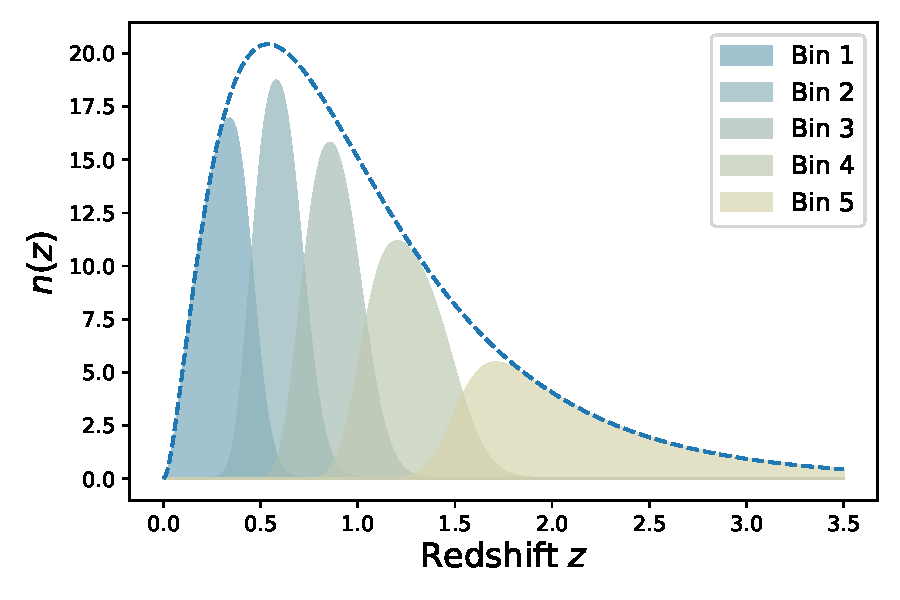
\includegraphics[width=\columnwidth]{figures/redshift_distribution_light.pdf}
    \caption{
     Source sample redshift distributions for each tomographic bin for LSST Y10. The number density on the y-axis is shown in arcmin$^2$.
    }
     \label{fig:redshift_distribution}
\end{figure}
%--------------------------------------------------------------------
% ############# PLOT CONVERGENCE MAPS  #############
%--------------------------------------------------------------------
\begin{figure}
    \begin{center}
    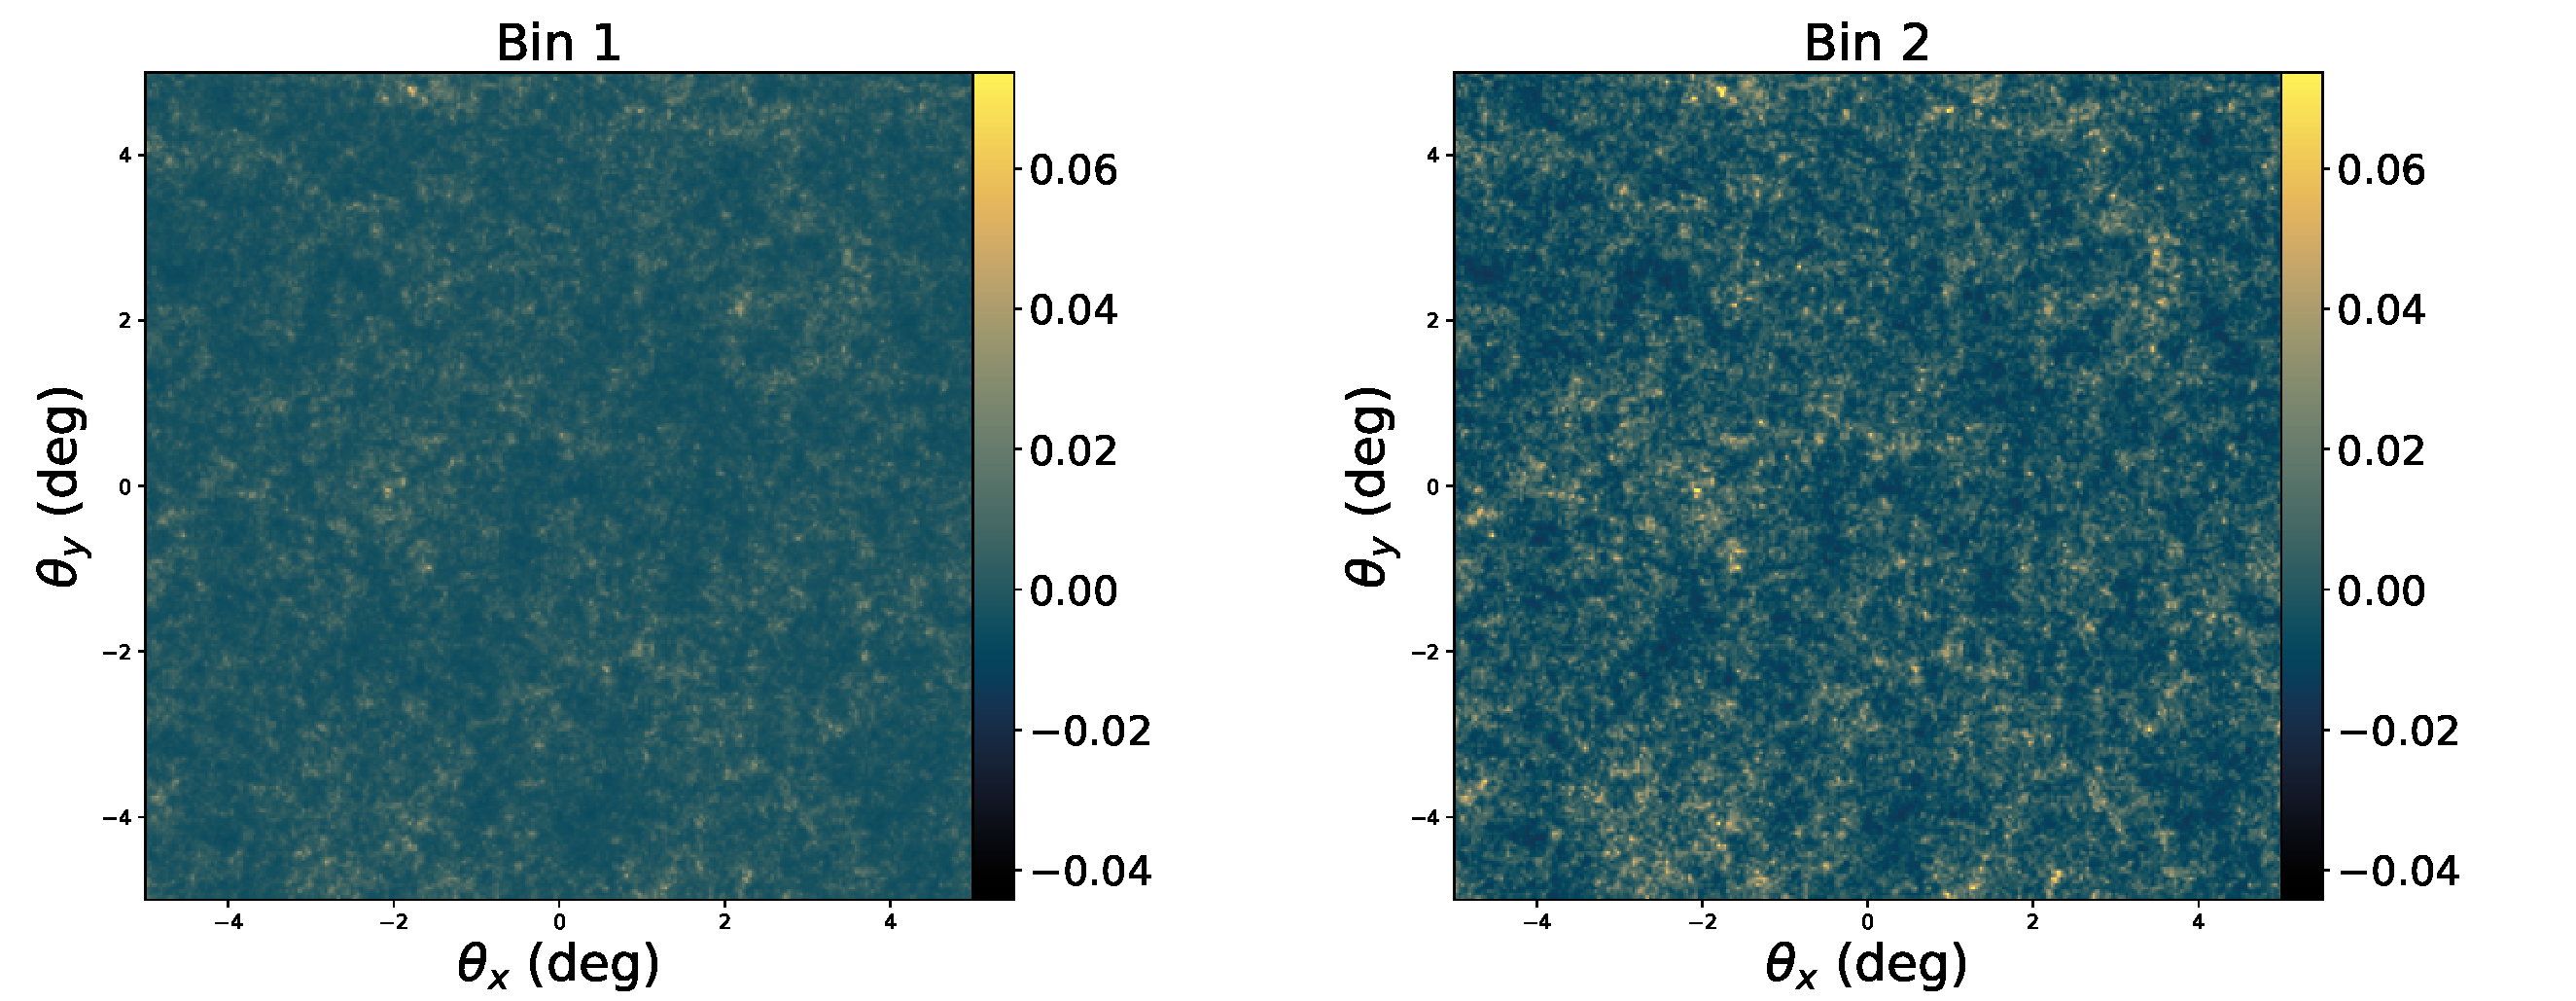
\includegraphics[width=\textwidth]{figures/bin1and2.pdf}
    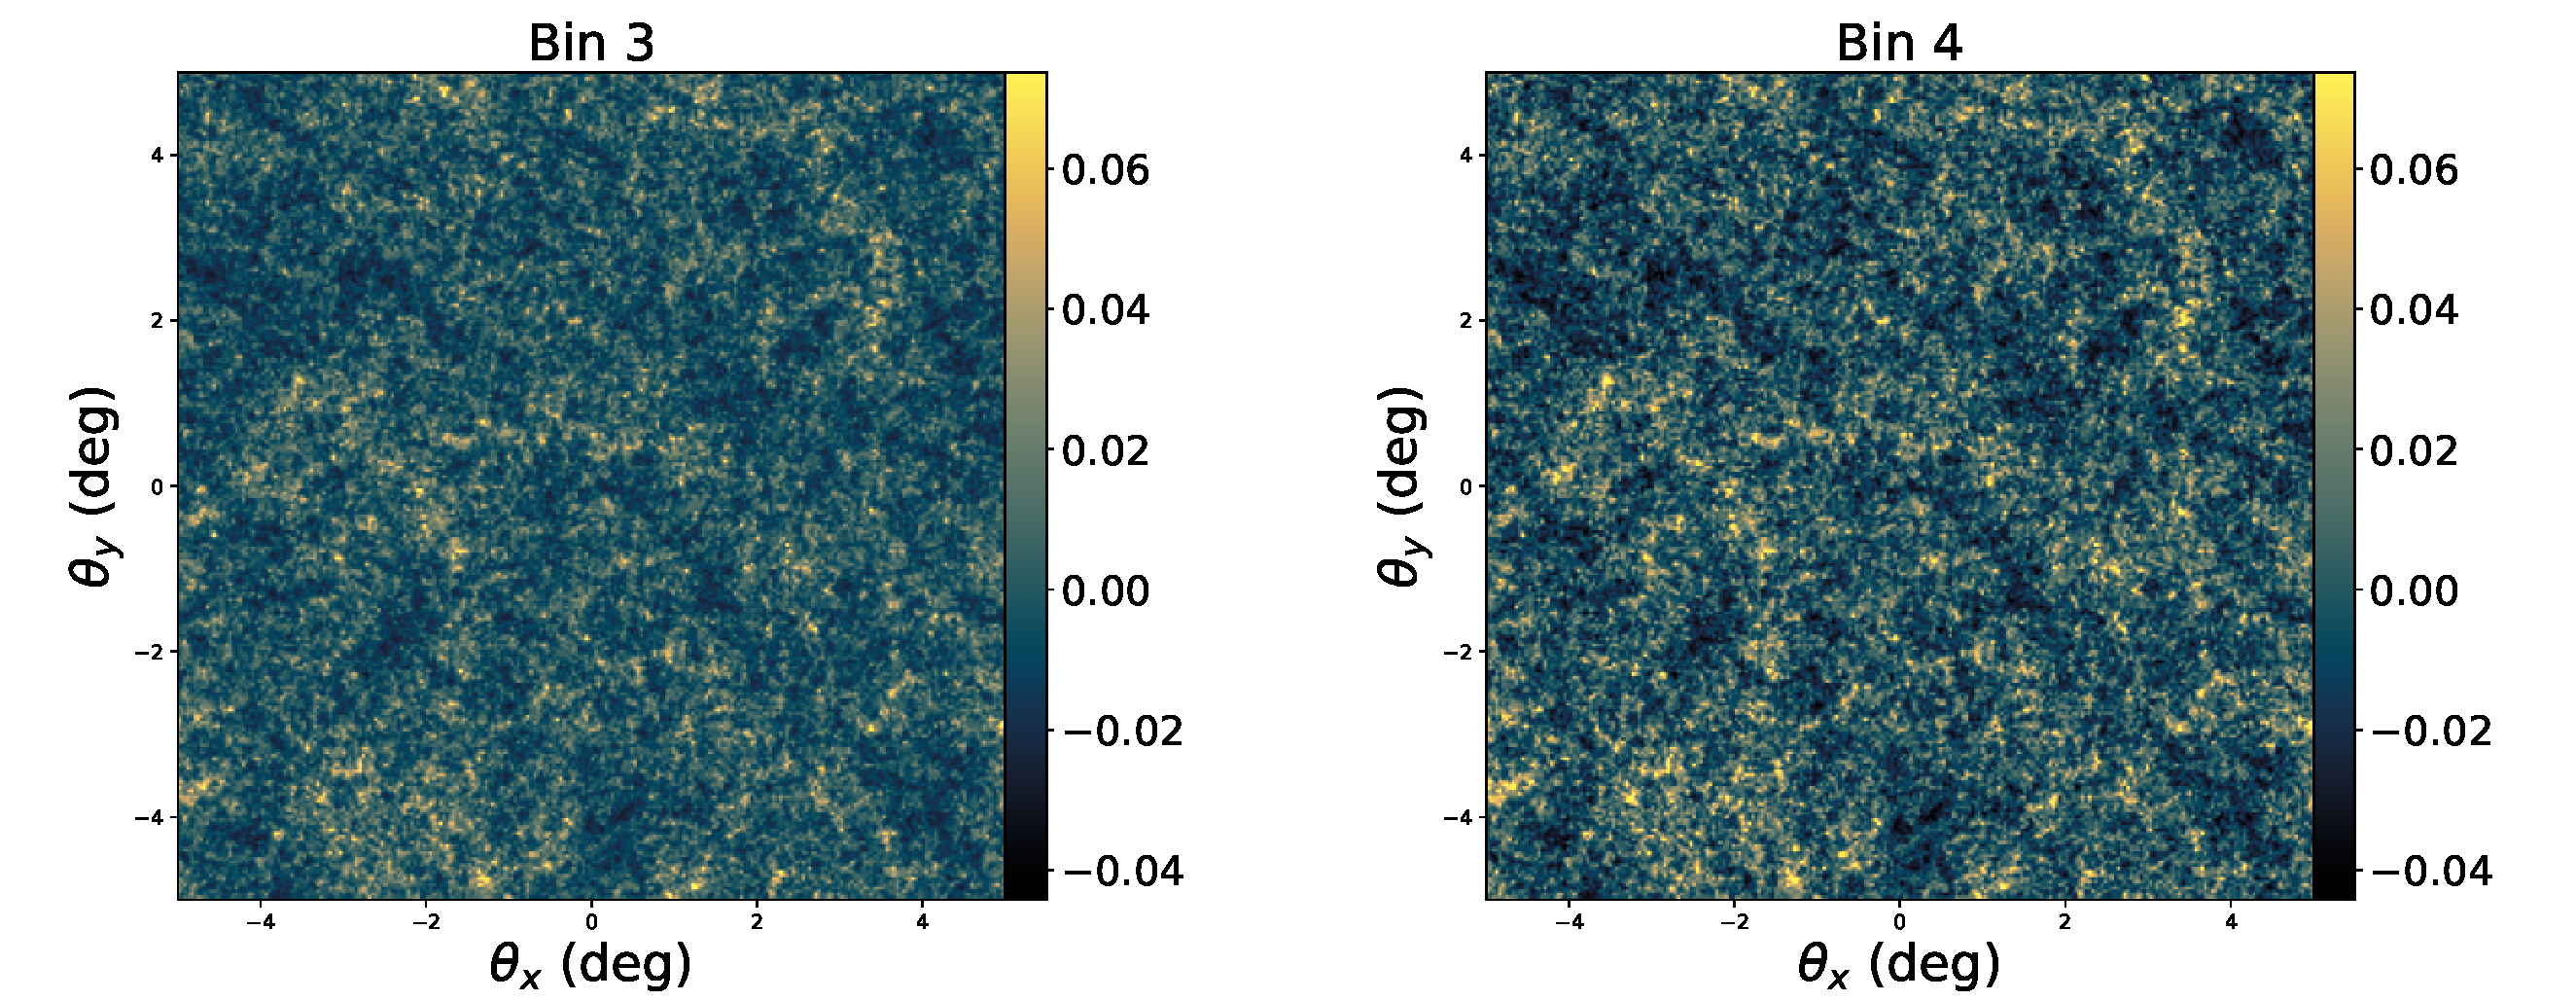
\includegraphics[width=\textwidth]{figures/bin3.pdf}
    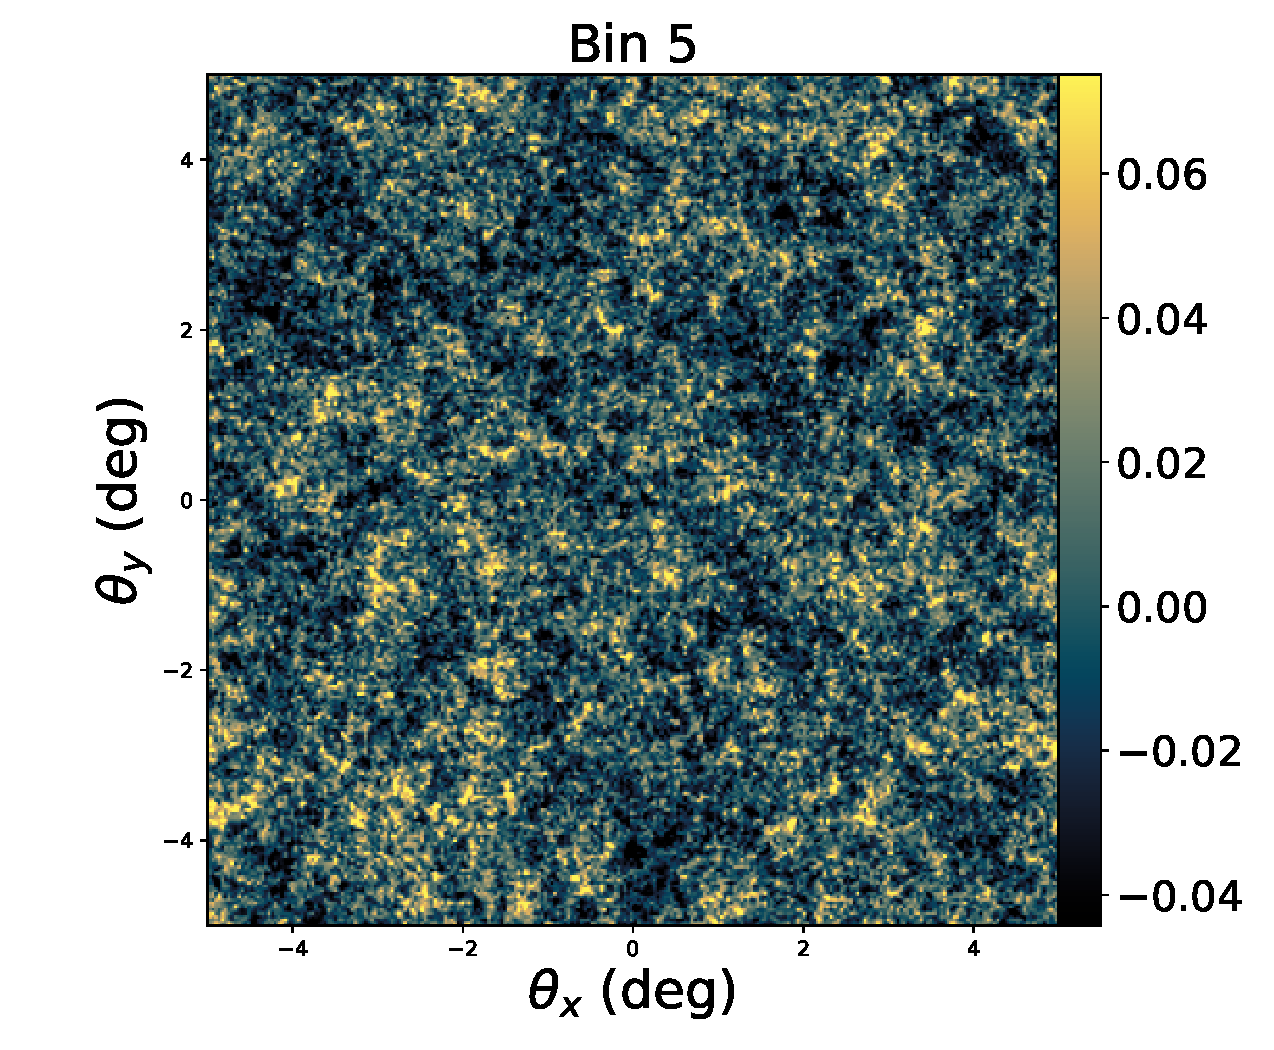
\includegraphics[width=0.5\textwidth]{figures/bin5.pdf}
    \caption{
     Example of convergence map simulated using the \texttt{SBILens} package.
    }
     \label{fig:convergence_maps}
     \end{center}
\end{figure}
%--------------------------------------------------------------------
% ############# PLOT CONVERGENCE MAPS  #############
%--------------------------------------------------------------------
\begin{figure*}
    \centering
    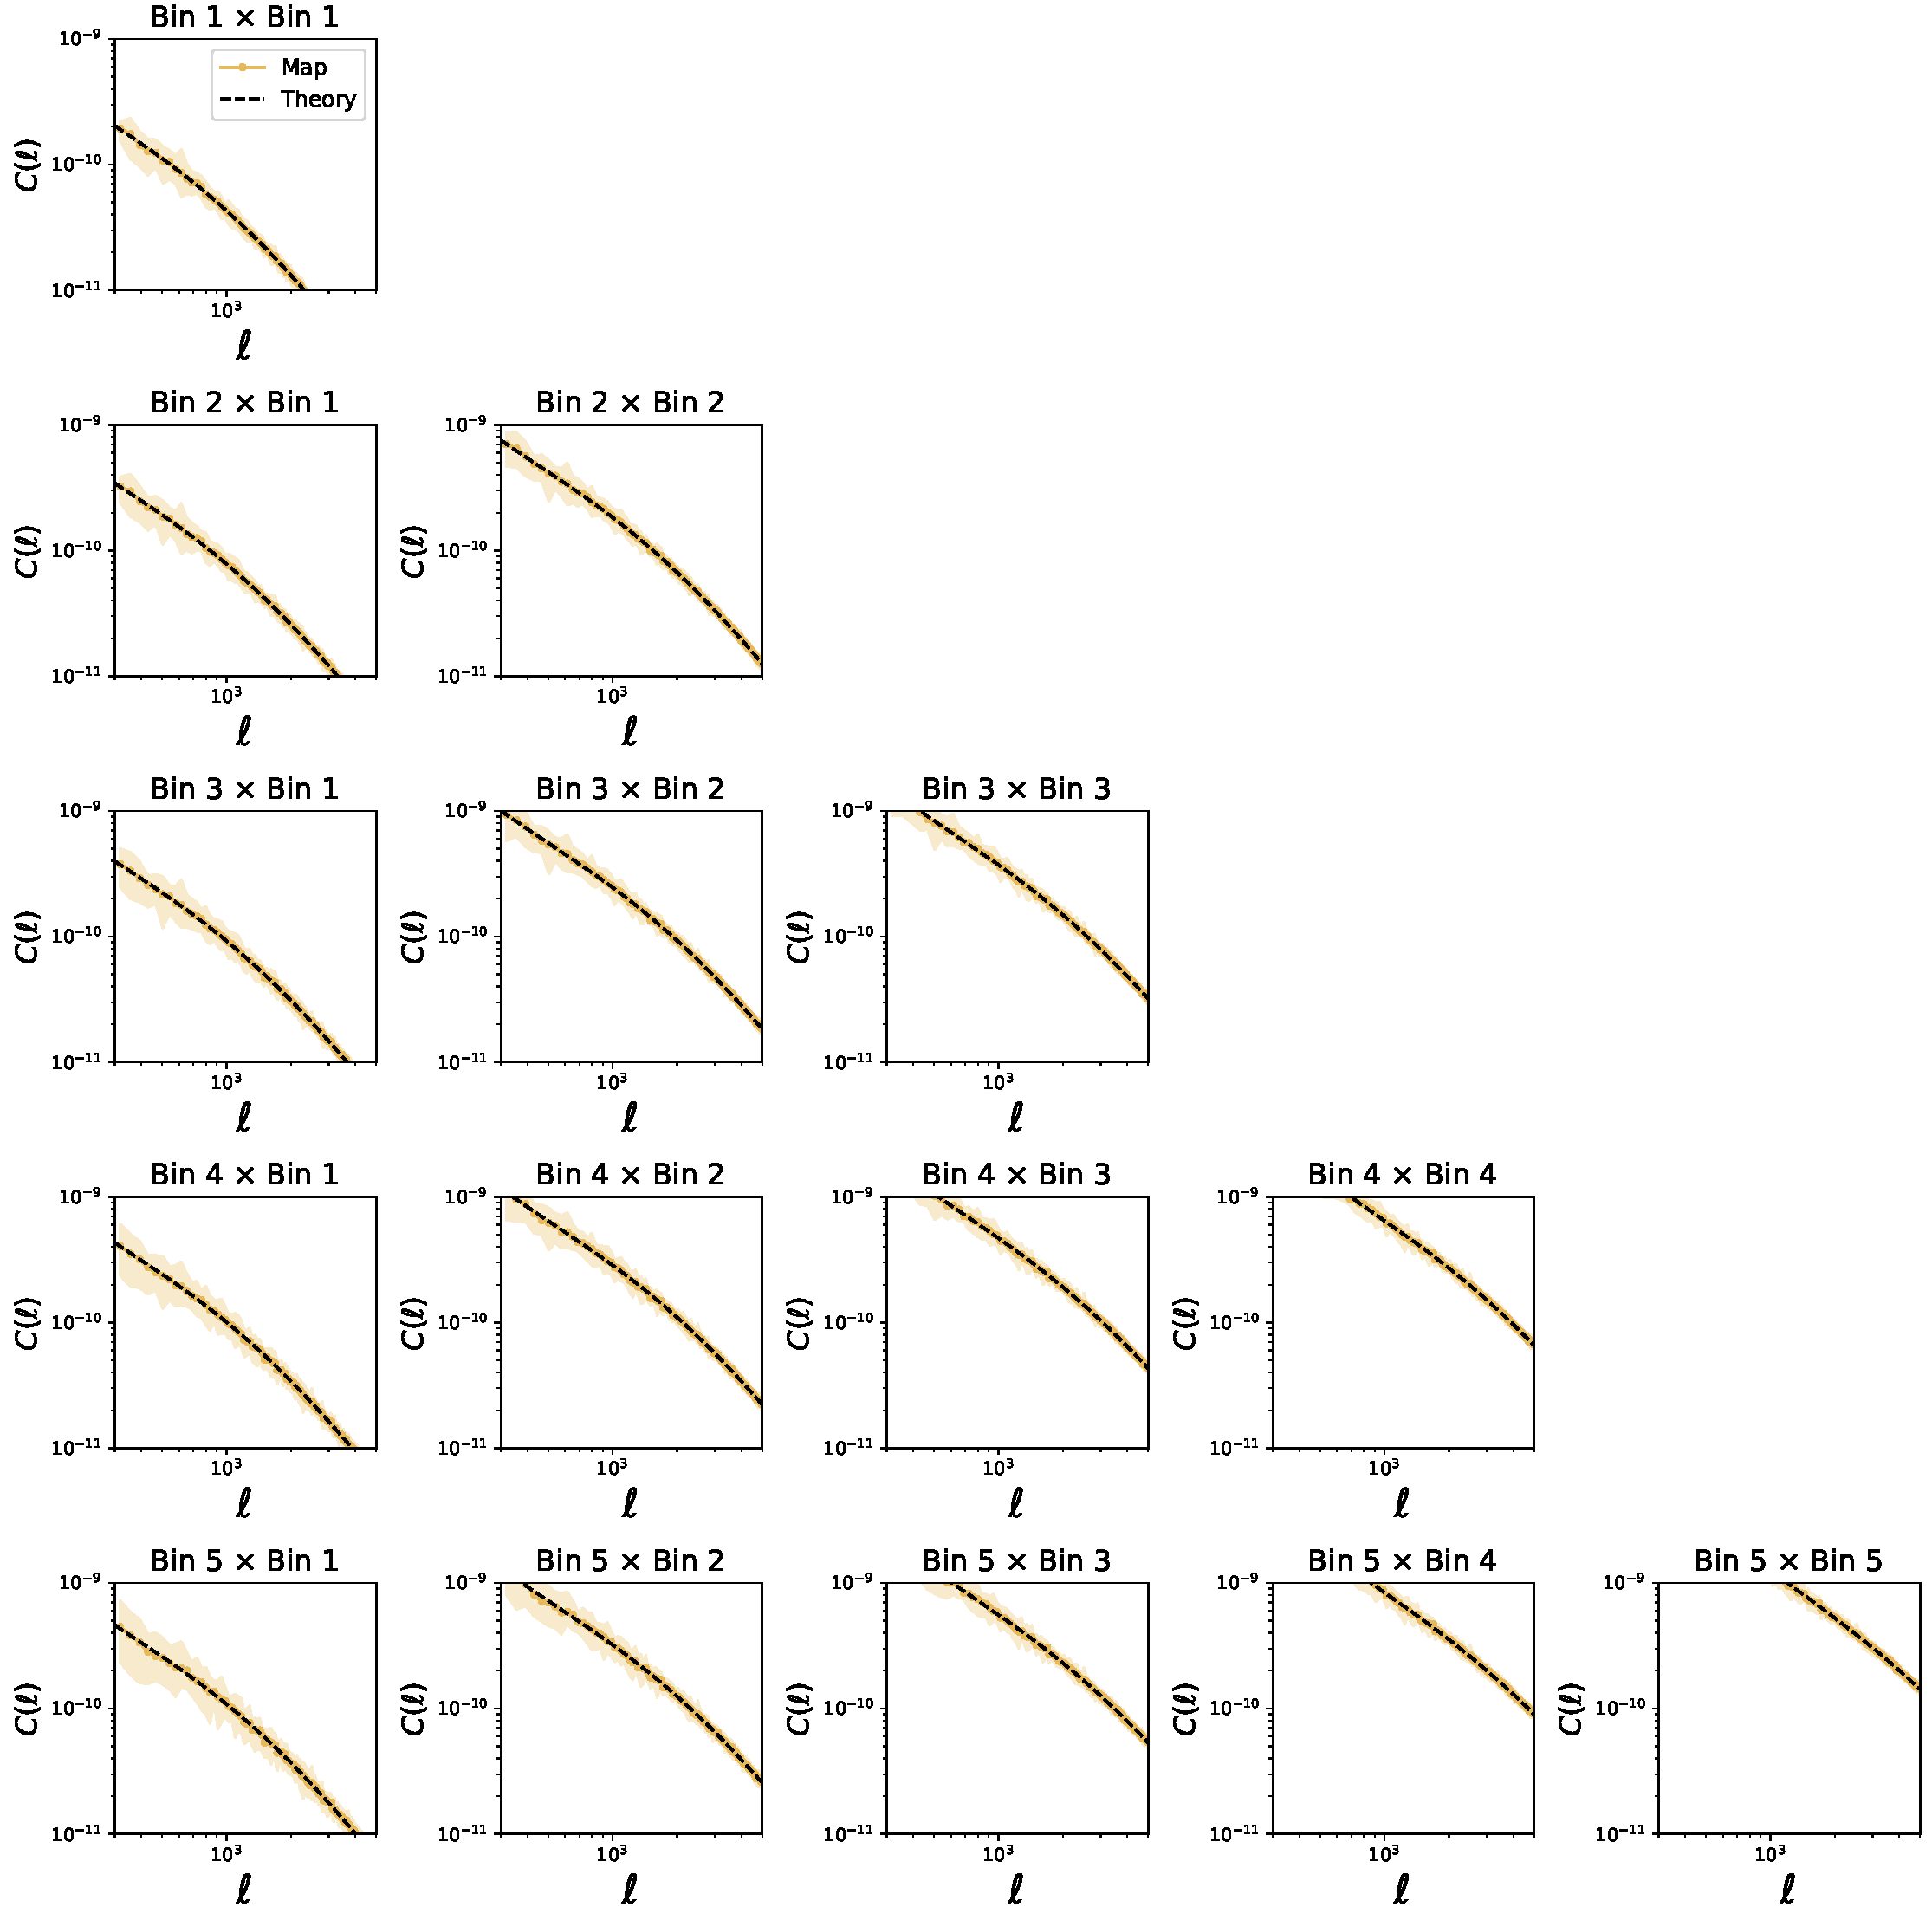
\includegraphics[width=\textwidth]{figures/psconvergencemaps.pdf}
    \caption{
    Convergence power spectra for different tomographic bin combinations. The solid yellow line shows the measurement from 20 simulated maps using the survey setting described in \autoref{Sec:the SBILens framework}, while the black dashed line shows the theoretical predictions computed using jax-cosmo. In this figure, the shaded regions represent the standard deviation from 20 independent map realizations.
    }
     \label{fig:psconvergence_maps}
\end{figure*}
%--------------------------------------------------------------------
%--------------------------------------------------------------------
%--------------------------------------------------------------------
%------------------------------------------------------------------
\section{Experiment}\label{Sec:experiment}
In the following section, we illustrate the inference strategy for the two approaches under investigation: the Bayesian forward modeling and the map-based inference based on the LFI.
Additionally, we conduct a power spectrum study. Indeed, as discussed in \autoref{Sec:Lognormal Modeling}, log-normal fields offer the advantage of rapidly generating convergent fields while accounting for non-Gaussianities. To emphasize this claim further, along with the full-field analysis, we include a power spectrum analysis. This analysis demonstrates that there is indeed a gain of information when adopting a full-field approach. \\
Finally, we provide a detailed overview of various neural compression strategies that differ in terms of the loss functions used to train the neural network.
%--------------------------------------------------------------------
%--------------------------------------------------------------------
%--------------------------------------------------------------------
\subsection{Explicit Inference}
%--------------------------------------------------------------------
%--------------------------------------------------------------------
%--------------------------------------------------------------------
\subsubsection{Full field with BHMs}
%--------------------------------------------------------------------
%--------------------------------------------------------------------
%--------------------------------------------------------------------
To construct the explicit map-based inference strategy in the Hierarchical Bayesian framework, we built a likelihood based on the data model described in \autoref{Sec:Lognormal Modeling}. 
As mentioned before, this means that the simulator serves as the physical model capable of generating the non-linear representation of the convergence map.

However, in practical terms, the measurement of convergence for each pixel and bin will differ from real observations due to noise. This is taken into consideration in the likelihood. Specifically, for LSST Y10, the number of galaxies for each pixel should be sufficiently high so that, according to the central limit theorem, we can assume the observation is characterized by Gaussian noise, with $\sigma_n^2=\sigma_e^2/N_s$, where $N_s$ represents the total number of source galaxies per bin and pixel. Given $\sigma_n^2$ the variance of this Gaussian likelihood, its negative log-form can be expressed as:
\begin{equation}
    \mathcal{L}(\bm{\theta})=
    \sum_i^{N_{pix}} \sum_{j}^{N_{bins}} \log{P(\kappa^{obs}_{i,j}|\kappa_{i,j},\bm{\theta})}
    =-\sum_i^{N_{pix}} \sum_{j}^{N_{bins}}\frac{[\kappa_{i,j}-\kappa^{obs}_{i,j}]^2}{2\sigma_n^2},
\end{equation}
where $\kappa^{obs}$ refers to the values of convergence from noise maps. \\
Since the full-field approach does not rely on any summary statistics, it typically leads to a high-dimensional problem, requiring more sophisticated statistical techniques. To sample the posterior distribution for $\bm{\theta}$, we use a Hamiltonian Monte Carlo (HMC) algorithm. 
Specifically, we employ the \texttt{NUTS} algorithm, an adaptive variant of HMC implemented in \href{https://github.com/pyro-ppl/numpyro}{\texttt{NumPyro}} \citep{phan2019composable, bingham2019pyro}, which uses the No U-Turn Sampler (NUTS, \citet{hoffman2014no}). \\
The HMC algorithm is particularly helpful in high-dimensional spaces where a large number of steps are required to effectively explore the space. It improves the sampling process by leveraging the information contained in the gradients to guide the sampling process. As the code is implemented in Jax, the gradients are accessible via automatic differentiation. 
%--------------------------------------------------------------------
%--------------------------------------------------------------------
%--------------------------------------------------------------------
\subsubsection{Power spectrum}
%--------------------------------------------------------------------
%--------------------------------------------------------------------
%--------------------------------------------------------------------
To obtain the probability distribution of the cosmological parameters using a summary-statistics method, we focus on the 2-point statistics, specifically, on the angular power spectra $C_{\ell}$.
We assume a Gaussian likelihood with a cosmology-independent covariance matrix:
\begin{equation}
    \mathcal{L}(\bm{\theta})=-\frac{1}{2}[\bm{d}-\bm{\mu}(\bm{\theta})]^{T}\bm{C}^{-1}[\bm{d}-\bm{\mu}(\bm{\theta})].
\end{equation}
To compute the expected theoretical predictions $\bm{\mu}(\bm{\theta})$ we use the public library \href{https://github.com/DifferentiableUniverseInitiative/jax_cosmo}{\texttt{jax-cosmo}} \citep{Campagne_2023}. 
 The Covariance matrix $\bm{C}$ of the observables is computed at the fiducial cosmology, presented in \autoref{tab:prior}, using the same theoretical library. Specifically, in {\texttt{jax-cosmo}}, the Gaussian covariance matrix is defined as:
\begin{equation}
    \text{Cov}(C_{\ell},C_{\ell'})=\frac{1}{f_{sky}(2 \ell+1)}\left(C_{\ell}+\frac{\sigma_{\epsilon}^2}{2n_s}\right)
\end{equation}
where $f_{sky}$ is the fraction of sky observed by the survey, and $n_s$ is the number density of galaxies. 
To obtain the data vector $\bm{d}$, containing the auto- and the cross-power spectra for each tomographic bin, we use the \href{https://lenstools.readthedocs.io/en/latest/lenstool} {\texttt{LensTools}} package \citep{2016A&C....17...73P} on a single noisy simulated map (our fiducial). 
To constrain the cosmological parameters, we sample from the posterior distribution using an HMC algorithm with adaptive step size, implemented in the TensorFlow Probability MCMC python package.
%--------------------------------------------------------------------
%--------------------------------------------------------------------
%--------------------------------------------------------------------
\subsection{Implicit Inference}
%--------------------------------------------------------------------
%--------------------------------------------------------------------
%--------------------------------------------------------------------
\subsubsection{Benchmark compression scheme}
To ensure the scalability of density estimation LFI in cases where forward simulations are computationally expensive, it becomes necessary to employ compression techniques that reduce the dimensionality of the data space and extract summary statistics. 
Specifically, we try to find a function $\bm{t}=F(\bm{x})$, where $\bm{t}$ represents low-dimensional summaries of the original data vector $\bm{x}$. The objective is to achieve a compression function $F(\bm{x})$ that maximizes the information while minimizing dimensionality. Previous studies \citep{heavens2000massive} have demonstrated that a compression scheme can be achieved where the dimension of the summaries dim($\bm{t}$) is equal to the dimension of the unknown parameters dim($\bm{\theta}$) without any loss of information at the Fisher level. Multiple approaches exist in an attempt to satisfy this condition. This section aims to provide an overview of the various neural compression-based methods employed in previous works.
%--------------------------------------------------------------------
\paragraph{\textcolor{violet}{Mean Square Error (MSE)}}
%--------------------------------------------------------------------
One of the commonly used techniques for training a Neural Network is by minimizing the $L_2$ norm or Mean Square Error (MSE).
This methods has been widely adopted in various previous studies  \citep{ribli2018improved, lu2022simultaneously, lu2023cosmological}, where the loss function is typically formulated as follows:
\begin{equation}
   \mathcal{L}=\frac{1}{N_{\theta}}(\bm{t}-\bm{\theta})^2.
\end{equation}
Here $N_{\theta}$ represents the number of cosmological parameters, $\bm{t}$ denotes the summary statistics, and $\bm{\theta}$ corresponds to the data vector of the cosmological parameters. 
However, it is important to note that this approach does not guarantee the recovery of maximally informative summary statistics. Indeed, minimizing the $L_{2}$ norm is equivalent to training the model to estimate the mean of the posterior distribution.  We prove this statement in \autoref{Sec:appendix_Mean Square Error}.
%--------------------------------------------------------------------
\paragraph{\textcolor{violet}{Maximum Absolute Error (MAE)}}
%--------------------------------------------------------------------
Another commonly used approach involves minimizing the $L_1$ norm or Mean Absolute Error (MAE). In this approach, the loss function is defined as:
\begin{equation}
    \mathcal{L}=|\bm{t}-\bm{\theta}|
\end{equation}
where $\bm{t}$ represents the summary statistics and $\bm{\theta}$ denotes the cosmological parameters.
In \autoref{Sec:appendix_Maximum Absolute Error}, we demonstrate that minimizing this loss function is equivalent to training the model to estimate the median of the posterior distribution. While extensively employed in various previous studies \citep{2018PhRvD..97j3515G, fluri2018cosmological, ribli2019weak}, similar to the previous consideration for the MSE, it is important to note that the effectiveness of this loss function in extracting sufficient statistics needs to be demonstrated.
%--------------------------------------------------------------------
\paragraph{\textcolor{violet}{Variational Mutual Information Maximization (VMIM)}}
%--------------------------------------------------------------------
The Variational Mutual Information Maximization (VMIM) technique was first introduced for cosmological inference problems by \citet{jeffrey2021likelihood}. This approach aims to maximize the mutual information $I(\bm{t}, \bm {\theta})$ between the cosmological parameters $\bm{\theta}$ and the summary statistics $\bm{t}$.
In the VMIM approach, the loss function is defined as:
\begin{equation}\label{Eq:Loss_vmim}
    \mathcal{L}=- \log{q(\bm {\theta} |F_{\bm {\varphi}}(\bm {x}) ; \bm{\varphi}')}.
\end{equation}
Here, $q(\bm {\theta} |F_{\bm {\varphi}}(\bm {x});\bm{\varphi'})$ represents a variational conditional distribution, where $\bm{\theta}$ corresponds to the data vector of the cosmological parameters, and $\bm{\varphi'}$ to the parameters characterizing the variational conditional distribution itself. $F_{\bm {\varphi}}$ denotes the compression network of parameter $\bm {\varphi}$, used to extract the summary statistics $\bm{t}$ from the original high-dimensional data vector $\bm{x}$, such that  $\bm{t}=F_{\bm {\varphi}}(\bm{x})$.
In order to understand the significance of this loss function, it is necessary to start by considering the mathematical definition of mutual information $I(\bm{t}, \bm {\theta})$:
\begin{align}\label{Eq:mutual_information}
    I(\bm{t}, \bm {\theta}) &= D_{KL}(p(\bm {t}, \bm {\theta})||p(\bm {t})p(\bm {\theta})) \\ \nonumber
    &= \int d\bm{\theta} d\bm{t} p(\bm t, \bm \theta)\log{\left( \frac{ p(\bm {t}, \bm {\theta})}{ p(\bm {t}) p(\bm {\theta})} \right)} \\ \nonumber
    &= \int d\bm{\theta} d\bm{t} p(\bm t, \bm {\theta})\log{\left( \frac{ p(\bm {\theta} | \bm {t} )}{ p(\bm {\theta})} \right)} \\ \nonumber
        &= \int d\bm{\theta} d\bm{t} p(\bm t, \bm {\theta})\log{p(\bm {\theta} | \bm {t} )} - \int d\bm{\theta}  d\bm{t} p(\bm t, \bm {\theta})\log{p(\bm {\theta})} \\ \nonumber
    &= \int d\bm{\theta} d\bm{t} p(\bm t, \bm {\theta})\log{p(\bm {\theta} | \bm {t} )} - \int d\bm{\theta} p(\bm {\theta})\log{p(\bm {\theta})} \\ \nonumber
    &= \mathbb{E}_{p(\bm {t}, \bm {\theta})} [\log{p(\bm {\theta} | \bm {t} )}]- \mathbb{E}_{p(\bm {\theta})} [\log{p(\bm {\theta})}] \\ \nonumber
    &= \mathbb{E}_{p(\bm {t}, \bm {\theta})} [\log{p(\bm {\theta} | \bm {t} )}]- H(\bm {\theta});
\end{align}
in the above equation, $D_{KL}$ is the Kullback-Leibler divergence \citep{kullback1951information}, $p(\bm {t}, \bm {\theta})$ is the joint probability distribution of summary statistics and cosmological parameters, and $H(\bm {\theta})$ represents the \textit{entropy} of the distribution of cosmological parameters.  
Essentially, mutual information measures the amount of information contained in the summary statistics $\bm t$ about the cosmological parameters $\bm \theta$.
The goal is to find the parameters of the network $\bm {\varphi}$ that maximize the mutual information between the summary and cosmological parameters:
\begin{equation}
   \bm {\varphi}^*= \operatorname*{argmax}_{\bm {\varphi}} I(F_{\bm {\varphi}}(\bm{x}), \bm {\theta}).
\end{equation}
However, the mutual information expressed in \autoref{Eq:mutual_information} is not tractable. To overcome this limitation, various approaches have been developed that rely on tractable bounds, enabling the training of deep neural networks to optimize mutual information. In this study, we adopt the same strategy used by \citet{jeffrey2021likelihood}, which involves using the variational lower bound \citep{barber2003information}:
\begin{equation}\label{Eq:variational_lower_bound}
    I(\bm{t}, \bm{\theta}) \ge \mathbb{E}_{p(\bm {t}, \bm {\theta})} [\log{q(\bm {\theta} |\bm{t} ; \bm{\varphi}')}]- H(\bm {\theta}).
\end{equation}
Here, the variational conditional distribution $\log{q(\bm {\theta} |\bm{t}; \bm{\varphi}')}$ is introduced to approximate the true posterior distribution $p(\bm{\theta}|\bm {t})$. 
As the entropy of the cosmological parameters remains constant for a fixed training set, the optimization problem based on the lower bound in \autoref{Eq:variational_lower_bound} can be formulated as:
\begin{equation}
    \operatorname*{argmax}_{\bm {\varphi}, \bm {\varphi}'}\mathbb{E}_{p(\bm {x}, \bm {\theta})} [\log{q(\bm {\theta} |F_{\bm {\varphi}}(\bm {x}) ; \bm{\varphi}')}], 
\end{equation}
yielding \autoref{Eq:Loss_vmim}.
%--------------------------------------------------------------------
\paragraph{\textcolor{violet}{Gaussian Negative Log-Likelihood (GNLL)}}
%--------------------------------------------------------------------
Recognizing that the uncertainty on different cosmological parameters will vary, a third
class of inverse variance weighted MSE was proposed in \cite{fluri2018cosmological} with the idea of
ensuring that each parameter contributes fairly to the overall loss by taking into account its uncertainty. The loss function typically takes the following form:
\begin{equation}
    \mathcal{L} = \frac{1}{2} \log(|\bm{\Sigma}|) + \frac{1}{2}(\bm{t} - \bm{\theta})^{\top} \Sigma^{-1} (\bm{t} - \bm{\theta}) 
\end{equation}
where $\bm{t}$ is the summary statistics and $\bm{\Sigma}$ is the covariance matrix representing the uncertainty on the cosmological parameters $\bm{\theta}$. Both $\bm{t}$ and $\bm{\Sigma}$ can be outputs of the compression network, i.e. $F_{\bm{\varphi}}(\bm{x})=(\bm{t}, \bm{\Sigma})$.

One recognizes here the expression of a Gaussian probability function, and this expression can thus be straightforwardly related to the VMIM case by simply assuming a Gaussian distribution as the variational approximation for the posterior $q(\bm{\theta} | \bm{x}) = \mathcal{N}(\bm{\theta}; \bm{t}, \bm{\Sigma})$.

This means that for this loss function:
\begin{itemize}
    \item The summary $\bm{t}$ extracted by the neural network is, similarly to the MSE case, only an estimate of the mean of 
    the posterior distribution, which is not guaranteed to be sufficient.
    \item Because of the Gaussian variational assumption, the variational posterior can potentially be biased with respect to the true posterior, and thus the mean of this Gaussian approximation may be biased with respect to the true posterior mean.
\end{itemize}
%--------------------------------------------------------------------
\paragraph{\textcolor{violet}
{Information Maximising Neural Networks (IMNNs)}}. 
A different approach has been proposed by \cite{charnock2018automatic} and further explored in \citet{Makinen_2021, Makinen_2022}. They implemented the Information Maximizing Neural Networks (IMNN), a neural network trained on forward simulations designed to learn optimal compression schemes, even in circumstances where the likelihood function is intractable or unknown.
Specifically, they proposed a new scheme to find optimal non-linear data summaries by using the Fisher information to train a neural network. 
Inspired by the MOPED algorithm \citep{heavens2000massive}, they aimed to find a transformation $f$ that maps the data to compressed summaries: $f: \textbf{x} \to \textbf{t}$ while conserving the Fisher information.  
The loss function takes the following form:
\begin{equation}\label{eq:loss_imnn}
    \mathcal{L} = -  |\text{det}(\textbf{F})|+ r_{\Sigma},
\end{equation}
where $\textbf{F}$ is the Fisher matrix, and $r_{\Sigma}$ is a regularization term typically dependent on the covariance matrix,  introduced to control the magnitude of the summaries.
Since computing the Fisher matrix requires a large number of simulations, they proceed as follows: a large number of simulations with the same fiducial cosmology but different initial random conditions are fed forwards through identical networks. The summaries from these simulations are combined to compute the covariance matrix. Additionally, the summaries from simulations created with different fixed cosmologies are used to calculate the derivative of the mean of the summary with respect to the parameter.\footnote{The method of finite differences is necessary when the framework in which the code is implemented does not support automatic differentiation.} Finally, the covariance and the mean derivatives are combined to obtain the Fisher matrix.

An application of this method in the context of weak lensing can be traced back to the work of \citet{fluri2021cosmological, fluri2022full}. Following \citet{charnock2018automatic}, they presented a compression approach that relies on the optimization of the Cramér-Rao bound. However, their approach does not assume that the summary follows a Gaussian likelihood. The loss function takes the form:
\begin{equation}\label{eq:loss_gfim}
\mathcal{L}=\log{\text{det}(\bm{\Sigma}_{\bm{\theta}}(\bm{t})})-2\log{\left|\text{det}\left(\frac{\partial \Psi_{\bm{\theta}}(\bm{t})}{\partial \bm{\theta}}\right)\right|},
\end{equation}
where $\bm{\Sigma}$ is the covariance matrix, and $\Psi_{\bm{\theta}}(\bm{t})=\mathbb{E}_{p(\bm {x}|\bm {\theta})}[\bm{t}]$.
This loss function is equivalent to the log-determinant of the inverse Fisher matrix used in \autoref{eq:loss_imnn}. \\
% \LM{TODO: condensed introduction; emphasize learning compression at single point; network learns score function which generalises smoothly away from fiducial \cite{Makinen_2021, Makinen_2022, Charnock_2018}, Wandelt (in prep.) 
% }
%--------------------------------------------------------------------
\subsection{Compression strategy}
%--------------------------------------------------------------------
The different compression strategies differ in the loss function employed during the training phase. For all of them, we use the same convolutional neural network architecture to build the compressor, specifically the ResNet-18, a deep ResNet architecture \citep{he2016deep}. The ResNet-18 is implemented using Haiku \citep{haiku2020github}, a Python deep learning library built on top of Jax.


While the different compression strategies share the same architecture, the training strategies for VMIM and GNLL differ significantly. To train the Neural compressor under VMIM and GNLL, we jointly optimize the weights $\bm{\varphi}$ of the Neural Network $F_{\bm{\varphi}}$ (the compressor) and the parameters $\bm{\varphi}'$ of the variational distribution $q_{\bm{\varphi}'}$. For VMIM, the variational distribution $q(\bm{\theta}|\bm{t};\bm{\varphi}')$ is modeled using a Normalizing Flow, while for GNLL, a Conditional Multivariate Gaussian estimator is employed. The Normalizing Flow used for the inference strategy is also adopted for the variational distribution required in the compression procedure.
For the Multivariate Gaussian estimator, we implement a three-layer neural network. The first two layers consist of fully connected layers with a Leaky Rectified Linear Unit activation function and a hyperbolic tangent activation function, respectively. The number of channels is increased to 256 and 128 for the first two layers, respectively. The last layer is a fully connected layer without an activation function, responsible for mapping the output of the first two layers to the desired output size (mean and covariance of the Gaussian distribution). \\
After training, we export the results of the neural compression $F_{\bm{\varphi}}$ but discard the results from the density estimator.
Indeed, as mentioned before, we perform the Likelihood-Free Inference (LFI) as a two-step procedure. This choice is motivated by the fact that it is difficult to train a very precise conditional density estimator when the compressor can still change from iteration to iteration. Hence, the choice to split the problem into two steps: first, the dimensionality reduction, where the density estimation part does not need to be perfect; second, the density estimation itself, which needs to be done very carefully now, but it is much easier because we are in low dimension.
%--------------------------------------------------------------------
%--------------------------------------------------------------------
%--------------------------------------------------------------------
%--------------------------------------------------------------------
\subsubsection{Inference strategy}\label{Sec:Inference_strategy}
%--------------------------------------------------------------------
%--------------------------------------------------------------------
By comparing the posteriors $p(\bm{\theta}| \bm{t})$ obtained with different compression strategies, we can assess the sensitivity of the results to the choice of the compression method. In particular, the more informative the summary statistics, the closer the posterior $p(\bm{\theta} | \bm{t})$ is to the true posterior $p(\bm{\theta} | \bm{x})$.  \\
As we have mentioned before, in the LFI context, the simulator is a black box that defines the likelihood distribution $p(\bm{x}|\bm{\theta})$ as an implicit distribution. We can sample from it, but we cannot directly evaluate it. The idea of Neural density Estimation is to introduce a parametric distribution model $\mathcal{P}_{\bm{\varphi}'}$ to approximate the implicit distribution $\mathcal{P}$. \\
In particular, we focus on Neural Posterior Estimation \citep{npe1, npe2, npe3}, i.e., we aim to directly approximate the posterior distribution. Specifically, we use a conditional Normalizing Flows \citep{nf1, nf2} to model the parametric conditional distribution $q_{\bm{\varphi}'} (\bm{\theta} | \bm{t})$, and we optimize the parameters ${\bm{\varphi}'}$ according to the following negative log-likelihood (NLL) loss function:
\begin{equation}\label{eq:nll}
    \mathcal{L}=- \log{q_{\bm{\varphi}'}(\bm{\theta}|\bm{t})}.
\end{equation}
In the limit of a large number of samples and sufficient flexibility, we obtain:
\begin{equation}
    q_{\bm{\varphi}'^\ast}(\bm{\theta} | \bm{t}) \approx p(\bm{\theta} | \bm{t})
\end{equation}
where we indicate with $\bm{\varphi}'^\ast$ the values of $\bm{\varphi}'$ minimizing \autoref{eq:nll}. \\
Finally, the target posterior $p(\bm{\theta} | \bm{t} = \bm{t_0})$ is approximated by $q_{\bm{\varphi}'^\ast}(\bm{\theta} | \bm{t} = \bm{t_0})$, where $\bm{t_0} = F_{\bm{\varphi}}(\bm{x_0})$, i.e., the compressed statistics from the fiducial convergence map $\bm{x_0}$ for a given compression strategy.

For each summary statistic, we approximate the posterior distribution using the same NF architecture, namely a RealNVP \citep{realnvp} with 4 coupling layers. The shift and the scale parameters are learned using a neural network with 2 layers of 128 neurons with Sigmoid-weighted Linear Units (SiLU) activation functions \citep{silu}. 
%--------------------------------------------------------------------
%--------------------------------------------------------------------
%--------------------------------------------------------------------
% ############# Begin Table BiblioSruvey  #############
%--------------------------------------------------------------------
\begin{table*}
    \begin{center}
        \begin{tabular}{ |p{5cm}|p{3cm}|p{5cm}| }
            \hline
            \makecell{\textbf{Reference}} &  \makecell{\textbf{Loss function}} &  \makecell{\textbf{Inference strategy}}  \\
            \hline
            \citet{2018PhRvD..97j3515G} & \makecell{MAE} &  \makecell{Likelihood-based analysis} \\
            \hline
            \citet{fluri2018cosmological} & \makecell{GNLL} & \makecell{Likelihood-based analysis}
            \\
            \hline     
             \rowcolor{lightgray}
                        \citet{fluri2019cosmological} &  \makecell{GNLL} &  \makecell{Likelihood-based analysis}
            \\
            \hline                    
                        \citet{ribli2019weak} & \makecell{MAE} & \makecell{Likelihood-based analysis}
            \\            
            \hline             
                        \citet{PhysRevD.102.123506} & \makecell{MAE} & \makecell{Likelihood-based analysis}
            \\
            \hline 
             \rowcolor{lightgray}
                        \citet{jeffrey2021likelihood} & 
                        \makecell{MSE \\ VMIM}
                        &  \makecell{Likelihood Free Inference \\ (Py-Delfi)} 
            \\            
            \hline             
                        \citet{fluri2021cosmological} &\makecell{IMNN} &   \makecell{Likelihood Free Inference \\ (GPABC)}  
            \\
            \hline      
             \rowcolor{lightgray}
                        \citet{fluri2022full} &  \makecell{IMNN} & \makecell{Likelihood Free Inference \\ (GPABC)} 
            \\            
            \hline 
                        \citet{lu2022simultaneously} & \makecell{MSE} & \makecell{Likelihood-based analysis}   
            \\           
            \hline 
                        \citet{kacprzak2022deeplss} & \makecell{GNLL}  & \makecell{Likelihood-based analysis} 
                      
            \\
            \hline 
             \rowcolor{lightgray}
                        \citet{lu2023cosmological} &  \makecell{MSE} & \makecell{Likelihood-based analysis} \\
                        
            \hline      
        \end{tabular}
        \caption{Table summarizing the different neural compression schemes used for weak lensing applications. The table includes all studies conducted within the context of implicit analysis (Likelihood-free) and standard Likelihood-based analysis. \\
        Abbreviations used in the Table: MSE-Mean Square Error; MAE-Maximum Absolute Error; GNLL- Gaussian Negative Log Likelihood; VMIM- Variational Mutual Information Maximization; IMNN- Information Maximizing Neural Networks; GPABC-Gaussian Processes Approximate Bayesian Computation.}
        \label{tab:biblio_survey}
    \end{center}
\end{table*}
%--------------------------------------------------------------------
% ############# End Table BiblioSruvey  #############
%--------------------------------------------------------------------
%--------------------------------------------------------------------
%--------------------------------------------------------------------
\section{Results}\label{Sec:results}
%--------------------------------------------------------------------
We present the results of the constraints on the full $\Lambda$CDM parameter space expected for a survey like LSST-Y10. The results are obtained using the simulation procedure outlined in \autoref{Sec:the SBILens framework} and the parameter inference strategy described in \autoref{Sec:Inference_strategy}.
We begin by analyzing the impact of the different compression strategies on the final cosmological constraints. Subsequently, we compare the outcomes of three different inference procedures: the 2-point statistics, the explicit full-field statistics, and the implicit full-field statistics using CNN summaries.
%--------------------------------------------------------------------
%--------------------------------------------------------------------
\subsection{Power spectrum and full-field statistics}
%--------------------------------------------------------------------
We now compare the constraining power of the three different approaches described in \autoref{Sec:experiment}: the standard two-point statistics and two map-based approaches, the explicit inference and the implicit inference strategy. 
As outlined before, our interest is to prove that the two map-based approaches lead to very comparable posterior distributions. We present the $68.3\%$ and $95.5\%$ confident regions from one fiducial map for the full $\Lambda$CDM parameters in \autoref{fig:contours_posterior_imp_ex_ps}. The contours obtained by the angular $C_{\ell}$ analysis are plotted in violet, the ones for the explicit inference (HMC) in orange, and those for the implicit inference (Normalizing Flow) in blue. 
We can see from the figure that the contours from the HMC-based inference and the Normalizing flow-based inference are remarkably similar.  We quantify the results by computing the Figure of Merit defined as follows:
\begin{equation}\label{Eq:Figure_of_merit}
    \text{FoM}_{\alpha \beta}=\sqrt{\text{det}(\Tilde{F}_{\alpha \beta})}.
\end{equation}
Here, $\alpha$ and $\beta$ represent a pair of cosmological parameters, and $\Tilde{F}_{\alpha \beta}$ refers to the marginalized Fisher matrix. We calculate $\Tilde{F}_{\alpha \beta}$ as the inverse of the parameter space covariance matrix $C_{\alpha \beta}$, which is estimated from the Normalizing flow sampling. 
Under the assumption of a Gaussian covariance, the FoM defined in \autoref{Eq:Figure_of_merit} is proportional to the inverse of the $2-\sigma$ contours in the 2-dimensional marginalized parameter space of the $\alpha$ and $\beta$ pair.
The results are presented in \autoref{tab:f_o_m}.
The remarkably strong agreement between the two posteriors confirms that the two map-based cosmology inference methods yield the same results. The ratio of their FoM, corresponding to 1.00, 1.04, 1.03, in the $(\Omega_c-\sigma_8); (\Omega_c-w_0); (\sigma_8-w_0$) plane, establishes the validity of the implicit inference strategy. \\
Confirming previous work, we note that $h$, $\Omega_b$, and $n_s$ result prior dominated and hence are constrained by none of the three approaches. 
Additionally, for the full-field strategies we find that the size of the contours is significantly smaller than the size for the prior distributions adopted, suggesting that the 
posterior on these parameters are not affected by the specific choice of prior.
Moreover, we find that the two-point statistic is suboptimal in constraining $\Omega_c$, $\sigma_8$, and $w_0$, while the two map-based approaches yield much tighter constraints on these parameters. 
We find that the map-based explicit and implicit strategies lead to an improvement in the figure of merit of $2.06\times$, 1.98$\times$, 2.28$\times$ and 2.06$\times$, 1.90$\times$, 2.22$\times$, respectively, in the $(\Omega_c-\sigma_8); (\Omega_c-w_0); (\sigma_8-w_0$) plane.
%--------------------------------------------------------------------
\subsection{Optimal compression strategy}
\autoref{fig:contours_posterior_diff_loss} shows our $68.3\%$ and $95.5\%$ constraints from one fiducial map using different compressed summaries.
We compare the constraints obtained from MSE (black contours), MAE (magenta contours), and VMIM (blue contours).
We note that the results obtained using different summaries are generally in agreement with each other, and there are no tensions present for any of the cosmological parameters. We report the marginalized summary constraints in \autoref{tab:summaries}. The results concern the cosmological parameters that are better constrained from weak lensing: $\Omega_c$, $\sigma_8$, $w_0$.
We note that the VMIM compressed summary statistics prefer values of $\Omega_c$, $\sigma_8$, and $w_0$ that are closer to our fiducial cosmology than those inferred by MSE and MAE. \\
To further quantify these outcomes, we consider the Figure of Merit described in \autoref{Eq:Figure_of_merit}. 
The results are presented in \autoref{tab:f_o_m}.
We can see that VMIM yields more precise measurements than MSE and MAE for all considered parameters.
In particular, the FoM of ($\Omega_c$, $\sigma_8$) is improved by $1.24\times$ and $1.1\times$ compared to MSE and MAE, respectively;  the FoM of ($\Omega_c$, $w_0$) is improved by $1.25\times$ and $1.17\times$ from the MSE and MAE; the FoM of ($\sigma_8$, $w_0$) is improved by $1.23\times$ and $1.15\times$ from the MSE and MAE.
%----------------------
%--------------------------------------------------------------------
%--------------------------------------------------------------------
% ############# PLOT CONTOURS HMC-SBI-PS  #############
%--------------------------------------------------------------------
\begin{figure*}
    \centering
        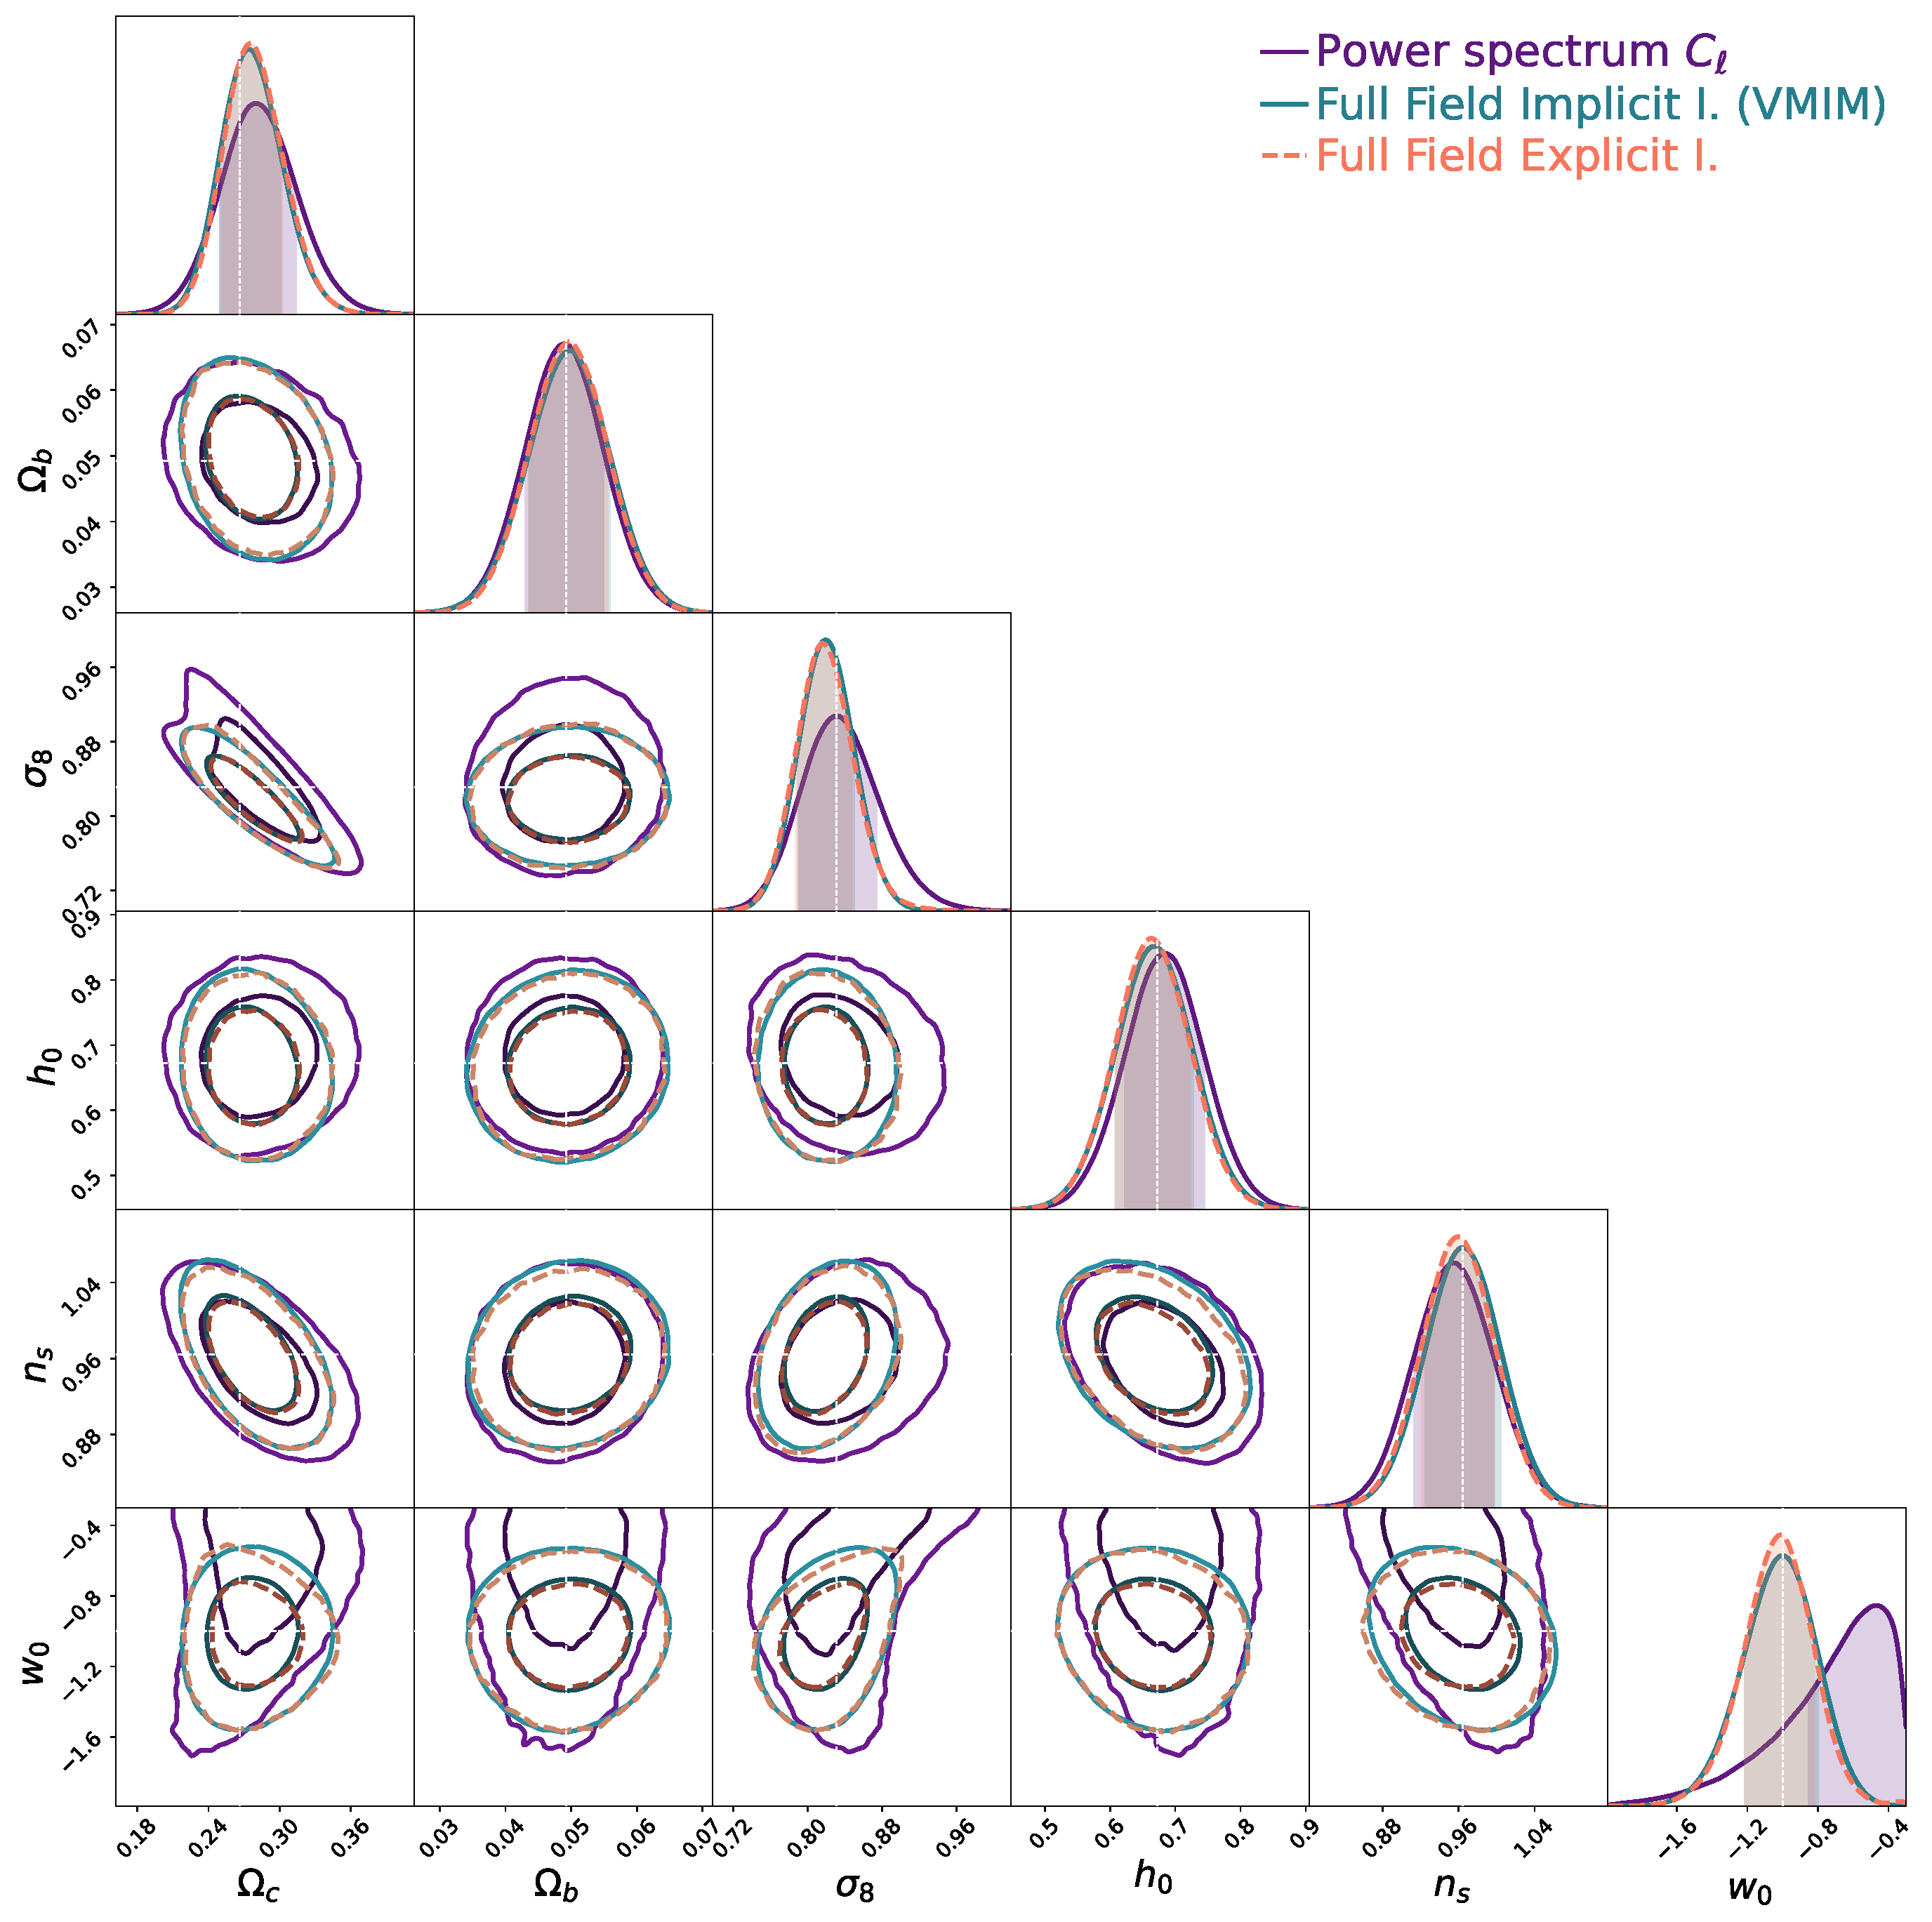
\includegraphics[width=\textwidth]{figures/contours_posterior_imp_ex_ps_dashed.pdf}
        \caption{
        Constraints on the $\Lambda$CDM parameter space as found in the LSST Y10 survey setup. The constraints are obtained by applying the $C_{\ell}$ (violet contours), the full field explicit inference (orange contours), and the full field implicit inference strategy (blue dashed contours), described in \autoref{Sec:experiment}.
        The contours show the $68\%$ and the $95\%$  confidence regions. The dashed white lines define the true parameter values.}
        \label{fig:contours_posterior_imp_ex_ps}
\end{figure*}
%-----------------------------------------------------------------
%--------------------------------------------------------------------
%--------------------------------------------------------------------
% ############# PLOT CONTOURS DIFFERENT LOSS FUNCTIONS  #############
%--------------------------------------------------------------------
\begin{figure*}
    \centering
        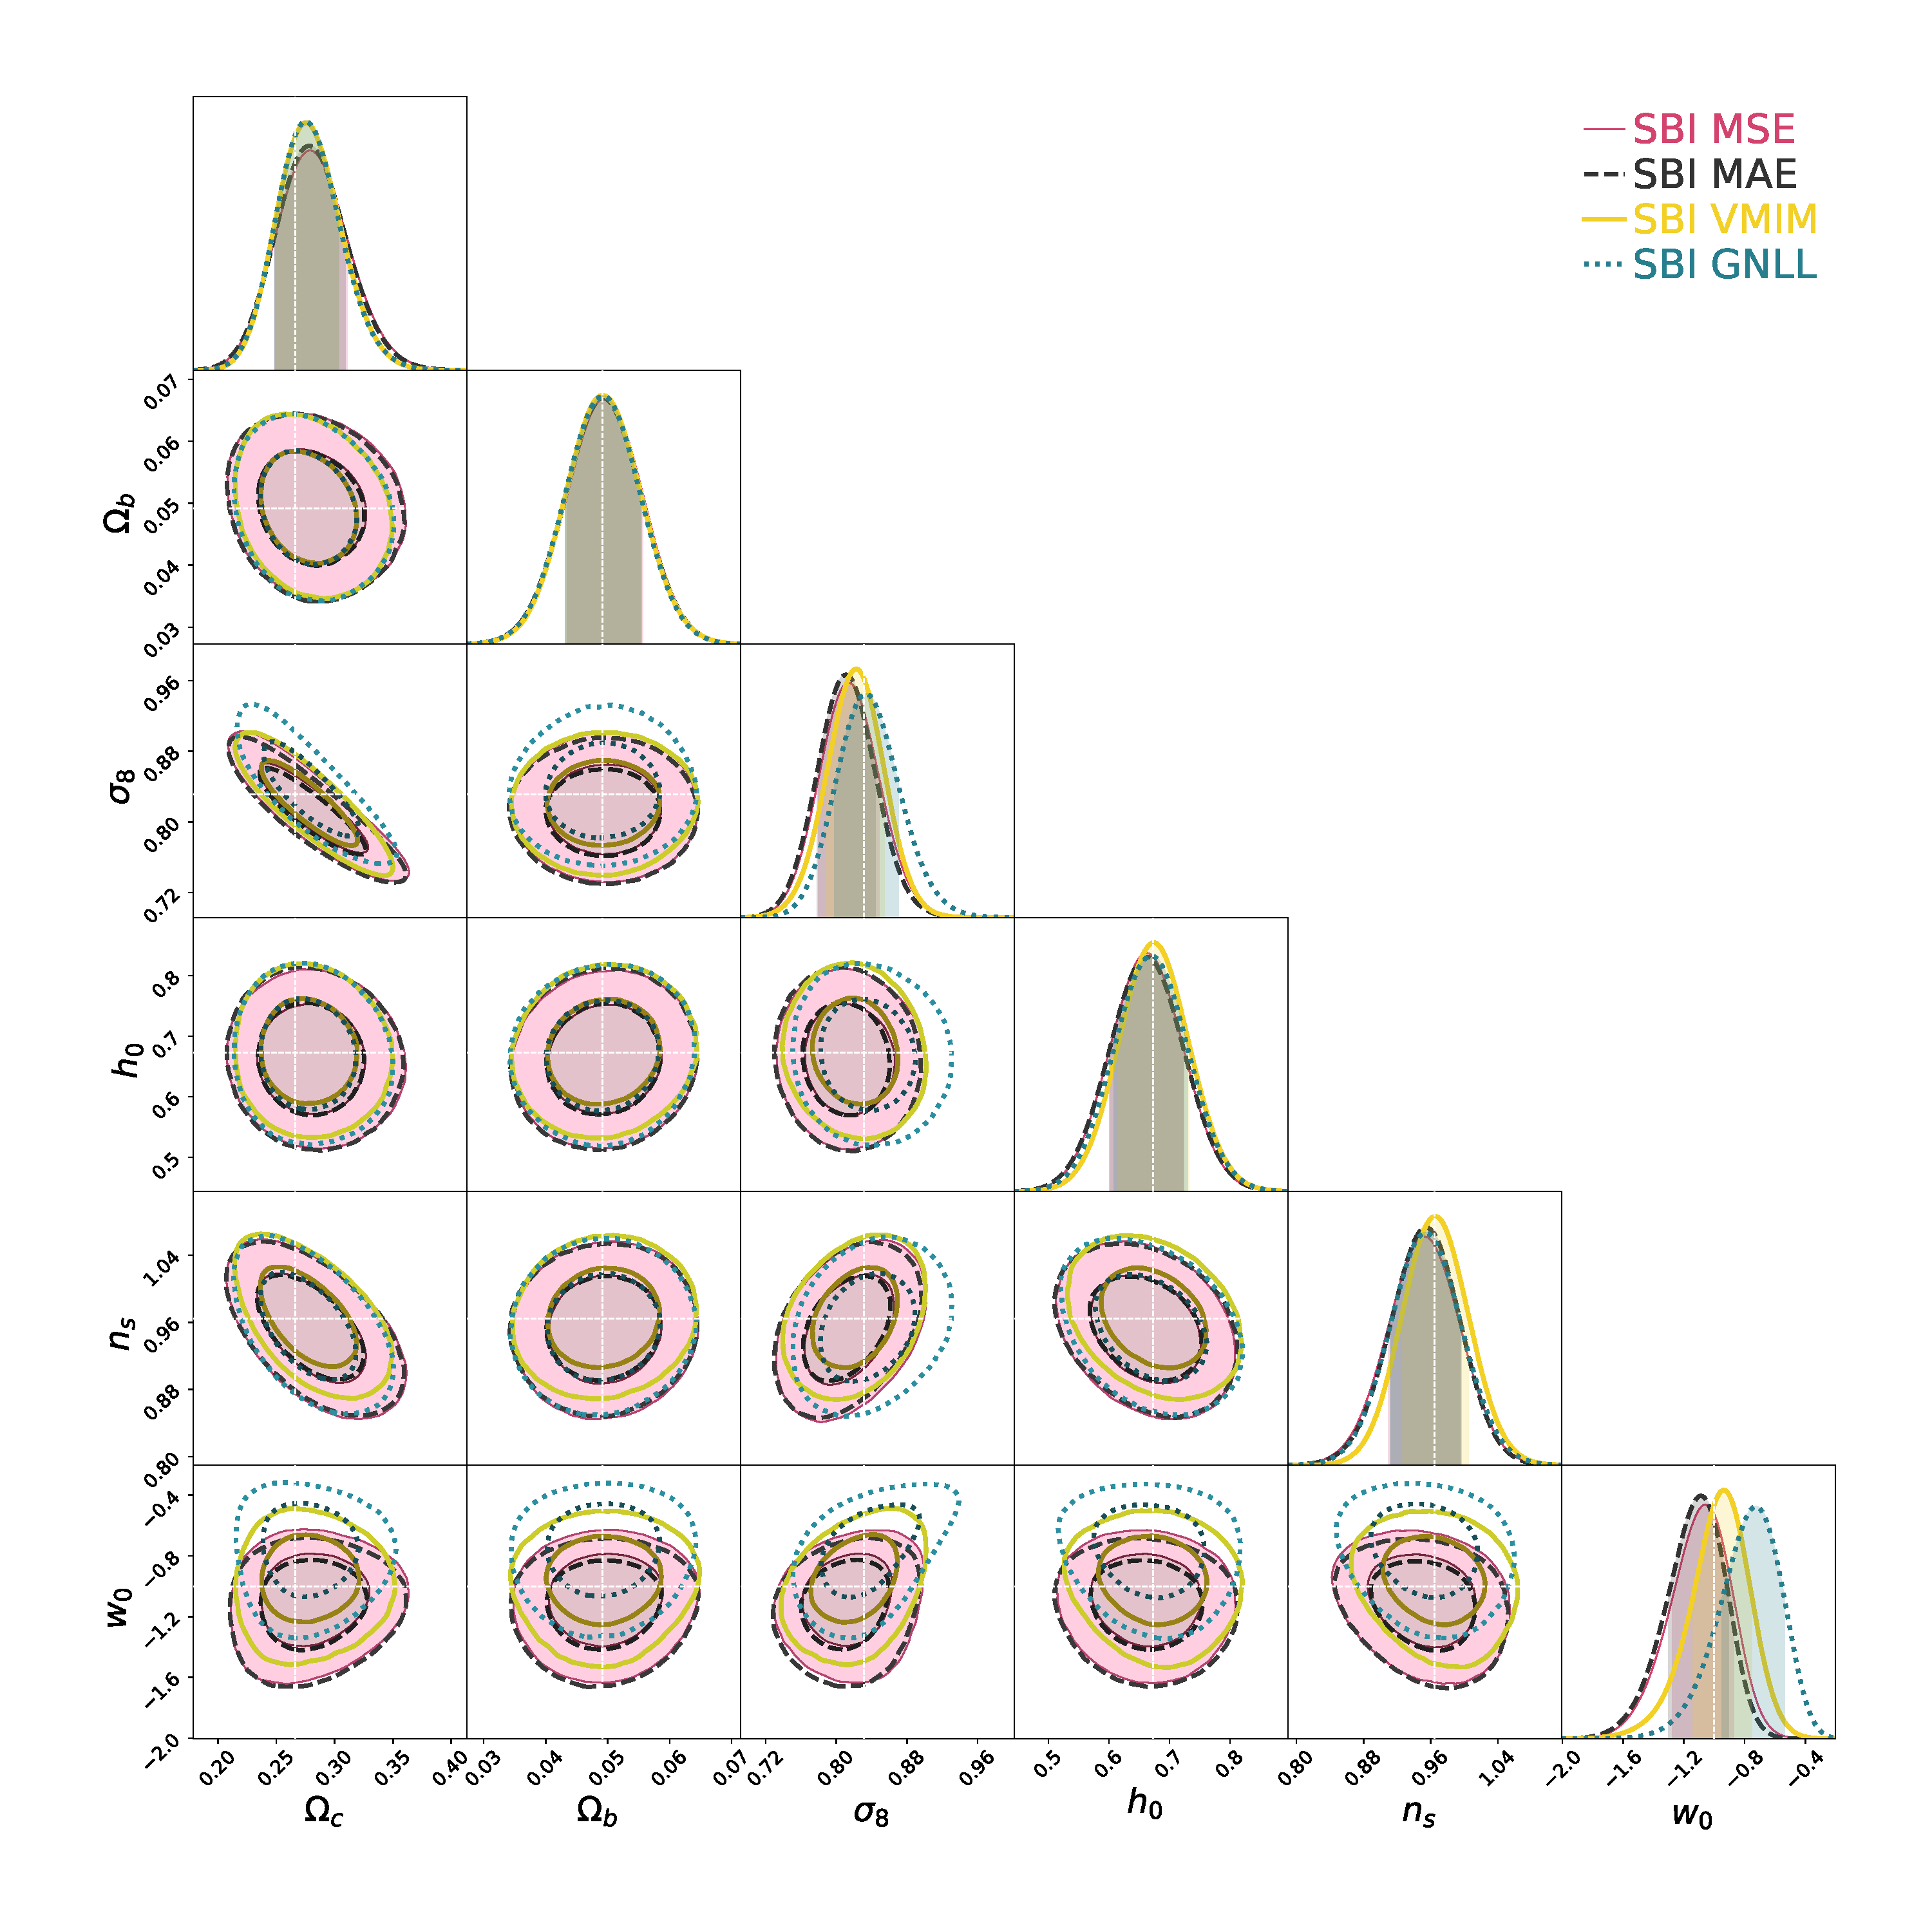
\includegraphics[width=\textwidth]{figures/contours_posterior_loss_dashed.pdf}
        \caption{
        Constraints on the $\Lambda$CDM parameter space as found in the LSST Y10 survey setup. The constraints are obtained from three CNN map compressed statistics: the MSE (black dashed contours), the MAE (magenta dashed contours), and VMIM (blue contours), described in \autoref{Sec:experiment}.
        The contours show the $68\%$ and the $95\%$  confidence regions. The dashed white lines define the true parameter values.}
        \label{fig:contours_posterior_diff_loss}
\end{figure*}
%--------------------------------------------------------------------
% ############# FIGURE OF MERIT TABLE  #############
%--------------------------------------------------------------------
\begin{table*}
    \begin{center}
        \begin{tabular}{lcccccc} 
            \hline
            FoM & $C_{\ell}$ & Full Field (HMC)&  VMIM & MSE & MAE & GNLL   \\
            \hline\hline
            $\Omega_c-  \sigma_8$ & 1222 & 2520 & 2526 & 2043 & 2316\\
            $\Omega_c-  w_0$      & 100  & 198  & 190  & 152  & 162\\
            $\sigma_8-  w_0$      & 77   & 176  & 171  & 139  & 149\\
            \hline
        \end{tabular}
        \caption{ Figure of Merit (FoM) for different inference strategies: the convergence power spectrum $C_{\ell}$, the HMC, the CNN map compressed statistics with the MSE, the VMIM, the MAE and the GNLL loss functions. The values of the figure of merit are inversely proportional to the area of the contours; the larger the FoM, the higher the constraining power.}
        \label{tab:f_o_m}
    \end{center}
\end{table*}
%--------------------------------------------------------------------
%  ############# SUMMARY TABLE  #############
%--------------------------------------------------------------------
\begin{table*}
    \begin{center}
        \begin{tabular}{|l|l|l|l|l|}
            \hline
             & VMIM & MSE & MAE &GNLL \\
            \hline
            \hline
            $\Omega_c$ & $0.274^{+0.026}_{-0.025}$  & $0.283^{+0.031}_{-0.029}$  & $0.279^{+0.030}_{-0.028}$ & \\
            \hline
            $\Omega_b$ & $ \left( 49.9^{+6.0}_{-6.4} \right) \times 10^{-3}$ &  $\left( 49.2\pm 6.1 \right) \times 10^{-3}$ &  $\left( 50.1^{+5.9}_{-6.1} \right) \times 10^{-3}$ &  \\
            \hline
            $\sigma_8$ & $0.819^{+0.031}_{-0.029}$  & $0.808^{+0.034}_{-0.032}$  &  $0.808^{+0.032}_{-0.030}$ &   \\
            \hline
            $w_0$      & $-1.00^{+0.20}_{-0.22}$  & $-1.13^{+0.23}_{-0.22}$ &   $-1.16\pm 0.22$  &  \\
            \hline
            $h_0$      & $0.666^{+0.061}_{-0.057}$ & $0.662^{+0.056}_{-0.057}$  & $0.664^{+0.056}_{-0.058}$  & \\
            \hline
            $n_s$      &  $0.963^{+0.041}_{-0.038}$ &  $0.956 \pm 0.041$ &  $0.955^{+0.039}_{-0.041}$  & \\
            \hline
        \end{tabular}
        \caption{Summary of the marginalized parameter distributions.}
        \label{tab:summaries}
  \end{center}
\end{table*}
%--------------------------------------------------------------------
%--------------------------------------------------------------------
\section{Summary and conclusions}\label{Sec:conclusion}
 In this work, we presented and compared two different map-based strategies for inferring cosmological parameters: the explicit full-field strategy, also known as Bayesian Hierarchical inference, based on an HMC sampler, and the implicit inference strategy, also known as Likelihood-Free Inference, based on a neural density estimator.


We start with a consideration: Deep learning approaches for implicit inference typically involve two steps. The first step is the automatic learning of an optimal low-dimensional summary statistic, and the second step is the use of a Neural Density Estimator in low dimensions to either build an estimate $P_{\bm{\varphi}}$ of the likelihood function $p(\bm{x}|\bm{\theta})$ (Neural Likelihood Estimation) or build an estimate $P_{\bm{\varphi}}$ of the posterior distribution $p(\bm{\theta}|\bm{x})$ (Neural Posterior Estimation). \\
Now, one can understand that both of these steps may potentially impact the final constraints on the parameters of interest. \\
Having said that, the main motivation for this work is to evaluate the impact of a given compression strategy on the final posterior distribution and, consequently, determine whether an optimal compression strategy exists. Furthermore, the aim is to demonstrate that by using this strategy, both implicit and explicit methods yield the same posterior. \\
To construct the forward model for explicit inference and simulate the mock data required to train the implicit model, we developed \href{https://github.com/DifferentiableUniverseInitiative/sbi_lens}{\url{SBILens}}, a Jax-based weak lensing simulator optimized for inference applications that need access to the model's derivatives. Our analysis is based on synthetic weak lensing data with five tomographic bins, mimicking a survey like LSST-Y10.


After providing an overview of the different compression strategies adopted in the literature for both Likelihood-Free Inference and likelihood-based inference strategies, we compared the impact of some of those on the final constraints on the cosmological parameters for a $\Lambda$CDM model. 
We found the following results:
\begin{enumerate}
    \item The marginalized summary statistics indicate that VMIM produces better results for $\Omega_c$, $w_0$, and $\sigma_8$ in terms of agreement with the fiducial value. However, it is important to note that the results from MSE and MAE are not in tension with the fiducial parameters.
    Furthermore, we quantified the outcomes by examining the figure of merit and found that VMIM provides more precise measurements compared to MSE and MAE.
    \item When using the VMIM to compress the original high-dimensional data, we compared the posterior obtained in the implicit inference framework with those obtained from Bayesian hierarchical modeling and the power spectrum. We demonstrate that both map-based approaches lead to a significant improvement in constraining $\Omega_c, w_0, \sigma_8$ compared to the 2-point statistics. However, $h, n_s, \Omega_b$ are not constrained by either and are prior-dominated.
    \item When using the VMIM to compress the original high-dimensional data the two methods, i.e., Bayesian hierarchical inference and Likelihood-free inference, lead to the same posterior distributions. 
\end{enumerate}

It is important to consider the potential limitations of the current implementation and highlight particular strategies for future extensions and applications of this project. In this work, we employed a physical model based on a lognormal prior, which is notably faster than simulation-based methods. Although we have shown that this description accounts for additional non-Gaussian information, as evidenced by the fact that we obtain different posteriors from the full-field and power spectrum methods, it is important to note that this is a good approximation for the convergence at intermediate scales but may not be appropriate for analyzing small scales. 
Furthermore, the lognormal shift parameters are computed using the \texttt{Cosmomentum} code \citep{friedrich2018density, friedrich2020primordial}, which employs perturbation theory. However, as mentioned by \citet{boruah2022map}, the perturbation theory-based approach may not provide accurate results at small scales.\footnote{However, as the main objective of this project is to compare the different inference strategies, we are not very concerned with the potential implications of this approximation at this stage.}

Additionally, we did not include any systemic in the current application, although previous studies demonstrated that the map-based approaches help to dramatically improve the constraints on systematic and cosmological parameters in the presence of these last. The main reason for this absence is mainly related to the difficulty of modeling systematic effects, like for example intrinsic alignment, in the lognormal description. \\
Hence, the natural next step will be to implement an N-body model as the physical model for the \texttt{SBILens} package. 
Specifically, we aim to work with the differentiable simulation we have presented in \citet{}. As mentioned in our previous work, the simulations can be improved and further developed by including additional systematics such as redshift uncertainties, baryonic feedback, and a more complicated intrinsic alignment model.
With these improvements, our model will be better suited to handle real cosmic shear data, allowing us to fully maximize the information gained from next-generation surveys. 
 
%--------------------------------------------------------------------
%--------------------------------------------------------------------
\begin{acknowledgements}
This work was granted access to the HPC/AI resources of IDRIS under the allocation 2022-AD011013922 made by GENCI.
\end{acknowledgements}
%--------------------------------------------------------------------
%              #########    START BIBLIO   #########
%--------------------------------------------------------------------
\bibliographystyle{aa} % style aa.bst
\bibliography{paper/biblio} 
%--------------------------------------------------------------------
%--------------------------------------------------------------------

%--------------------------------------------------------------------
%              #########    START APPENDIX   #########
%--------------------------------------------------------------------
\begin{appendix}
\section{Mean Square Error (MSE)}\label{Sec:appendix_Mean Square Error}
In this section, we demonstrate that minimizing the $L_2$ norm is equivalent to training the model to estimate the mean of the posterior distribution. Namely:
\begin{equation}\label{Eq:mean_mse}
\left \langle \bm {\theta} \right \rangle_{p(\bm {\theta}|\bm{x})}=\operatorname*{argmin}_{F(\bm{x})}\mathbb{E}_{p(\bm {\theta}|\bm {x})}[\left\Vert \bm {\theta}-F(\bm{x})
 \right \Vert_{2}^{2}],
\end{equation}
where the posterior mean $\left \langle \bm {\theta} \right \rangle_{p(\bm {\theta}|\bm{x})}$, is calculated as follows:
\begin{equation}\label{Eq:mean_pos}
     \left \langle \bm {\theta} \right \rangle_{p(\bm {\theta}|\bm{x})}= \mathbb{E}_{p(\bm {\theta}|\bm {x})}[\bm {\theta}].
\end{equation}
To demonstrate this statement, we need to minimize the expected value of the $L_2$ norm with respect to $F(\bm{x})$. Let us consider its derivative:
\begin{align}\label{Eq:moment_1}
   & \frac{\partial}{\partial F(\bm{x}) }  \mathbb{E}_{p(\bm {\theta}|\bm{x}))}[(\bm {\theta}-F(\bm{x}))^2] =  \\
    &
    \frac{\partial}{\partial F(\bm{x}) }  \mathbb{E}_{p(\bm {\theta}|\bm {x})}[\bm {\theta}^2+F(\bm{x})^2-2\bm {\theta}F(\bm{x})] = \nonumber \\
    &
    \frac{\partial}{\partial F(\bm{x}) }  [
    \mathbb{E}_{p(\bm {\theta}|\bm {x})}[\bm {\theta}^2]+F(\bm{x})^2-2F(\bm{x})\mathbb{E}_{p(\bm {\theta}|\bm {x})}[\bm {\theta}]]= \nonumber \\
    &2F(\bm{x})-2 \mathbb{E}_{p(\bm {\theta}|\bm {x})}[\bm {\theta}]. \nonumber
\end{align}
Setting it equal to zero, we obtain the critical value:
\begin{equation}\label{Eq:minimum_mean}
    F(\bm{x})= \mathbb{E}_{p(\bm {\theta}|\bm {x})}[\bm {\theta}]. 
\end{equation}
Considering the second-order derivative:
\begin{equation}
   \frac{\partial^2}{\partial^2 F(\bm{x})}  \mathbb{E}_{p(\bm {\theta}|\bm {x})}[(\bm {\theta}-F(\bm{x}))^2]=2>0, 
\end{equation}
we can assert that this critical value is also a minimum. \\
From \autoref{Eq:minimum_mean} and \autoref{Eq:mean_pos}, we obtain \autoref{Eq:mean_mse}.
%--------------------------------------------------------------------
\section{Maximum Absolute Error (MAE)}\label{Sec:appendix_Maximum Absolute Error}
In this section, we demonstrate that minimizing the $L_1$ norm is equivalent to training the model to estimate the median of the posterior distribution.
Namely:
\begin{equation}\label{Eq:median_mae}
 \bm {\theta}^M_{p(\bm {\theta}|\bm{x})}=\operatorname*{argmin}_{F(\bm{x})}\mathbb{E}_{p(\bm {\theta}|\bm {x})}[| \bm {\theta}-F(\bm{x})|].
\end{equation}
By definition, the median of a one-dimensional\footnote{For notational simplicity, we demonstrate this statement in one dimension; the generalization to N-dimensions is straightforward.} probability density function $p(x)$ is a real number $m$ that satisfies:
\begin{equation}\label{Eq:definition_median}
\int_{\infty}^{m} p(x)dx=\int_{m}^{\infty}p(x)dx=\frac{1}{2}.
\end{equation}
The expectation value of the maximum absolute error is defined as:
\begin{equation}
    \mathbb{E}_{p(x)}[|x-m|]= \int_{\infty}^{\infty}p(x)|x-m|dx  
\end{equation}
which can be decomposed as
\begin{equation}
        \int_{\infty}^{m}p(x)|x-m|dx +\int_{m}^{\infty}p(x)|x-m|dx .
\end{equation}
To minimize this function with respect to $m$, we need to compute its derivative:
\begin{equation}\label{Eq:absolute_median}
    \frac{d\mathbb{E}[|x-m|]}{dm}=
    \frac{d}{dm}\int_{\infty}^{m}p(x)|x-m|dx +\frac{d}{dm}\int_{m}^{\infty}p(x)|x-m|dx. 
\end{equation}
Considering that $|x-m|=(x-m)$ for $m\le x$ and $|x-m|=(m-x)$ $m\ge x$, 
we can write \autoref{Eq:absolute_median} as:
\begin{equation}
    \frac{d\mathbb{E}[|x-m|]}{dm}=
    \frac{d}{dm}\int_{\infty}^{m}p(x)(m-x)dx +\frac{d}{dm}\int_{m}^{\infty}p(x)(x-m)dx .
\end{equation}
Using the Leibniz integral rule, we get:
\begin{align}
    &\frac{d\mathbb{E}[|x-m|]}{dm}= \\
    &
    p(x)(m-m)\frac{dm}{dm}+\int_{\infty}^{m}\frac{\partial}{\partial m}[p(x)(m-x)]dx + \nonumber \\
    & - p(x)(m-m)\frac{dm}{dm}+\int_{m}^{\infty}\frac{\partial}{\partial m}[p(x)(m-x)]dx \nonumber .
\end{align}
Setting the derivative to zero, we obtain:
\begin{equation}
    \frac{d\mathbb{E}[|x-m|]}{dm}= \int_{\infty}^{m} p(x)dx-\int_{m}^{\infty}p(x)dx =0.
\end{equation}
Thus,
\begin{equation}
\int_{\infty}^{m} p(x)dx=\int_{m}^{\infty}p(x)dx .
\end{equation}
Considering that
\begin{equation}
\int_{\infty}^{m} p(x)dx+\int_{m}^{\infty}p(x)dx=1,
\end{equation}
we obtain \autoref{Eq:definition_median}.
%--------------------------------------------------------------------
%              #########    END APPENDIX   #########
%--------------------------------------------------------------------
\end{appendix}
\end{document}